\documentclass[a4paper,cleardoubleempty,BCOR1cm]{scrbook}
% use to waste space:
% \documentclass[12pt,a4paper]{article}

% if you have this style and like it.
%\documentclass{acmsiggraph}
%\documentclass[review]{acmsiggraph}      % review
%\documentclass[widereview]{acmsiggraph}  % wide-spaced review
%\documentclass[preprint]{acmsiggraph}    % preprint

% define a \comment{this is a comment which can have linebreaks in it}
\newcommand{\comment}[1]{}
% \newcommand{\todo}[1]{\marginpar{\bf{#1}}}
\newcommand{\todo}[1]{{\color{red}\bf{TODO: #1}}}

\usepackage{mathptmx}
\usepackage[pdftex]{graphicx}
\usepackage[pdftex]{color}
\definecolor{rot}{RGB}{165,30,55} %rote Farbe
\graphicspath{{./images/}}
\usepackage{parskip}
\usepackage{amsmath}
\usepackage{dsfont}
\usepackage{pxfonts}
\usepackage{apacite}

\usepackage[T1]{fontenc}
\usepackage{textcomp}

% comment these two lines out if you don't want minion/myriad fonts.
%\usepackage[minionint,mathlf]{MinionPro}
%\renewcommand{\sfdefault}{Myriad-LF}
%\usepackage{Myriad}

% no page number on float pages, fixes problems with overlarge diagrams.
\usepackage{fancyhdr}
\pagestyle{fancy}
%\lhead{}
%\chead{}
%\rhead{}
%\lfoot{}
\fancyhf{}
\fancyhead[EL]{\nouppercase{\leftmark}}
\fancyhead[OR]{\nouppercase{\rightmark}}
\cfoot{}
%\fancyfoot[EL]{\iffloatpage{}{\thepage}}
%\fancyfoot[OR]{\iffloatpage{}{\thepage}}
\fancyfoot[EL]{\thepage}
\fancyfoot[OR]{\thepage}
\renewcommand{\headrulewidth}{0pt}
\renewcommand{\footrulewidth}{0pt}

\usepackage{natbib}		% textual referencing
%\usepackage[numbers,super]{natbib}	% nice superscripts
%\bibliographystyle{chicago}	% shitty
%\bibliographystyle{alpha}	% abbr names and year in \cite
\bibliographystyle{apacite}  % not working, only with natbib(?)
%\bibliographystyle{agsm}	% australian, need natbib
%\bibliographystyle{kluwer}	% need natbib
%\bibliographystyle{apalike}	% lengthly
%\bibliographystyle{abbrv}	% minimal?

% use for german line breaking:
%\usepackage[ngerman]{babel}
\usepackage[T1]{fontenc}
\usepackage[utf8x]{inputenc}

% avoid us-style text color destruction:
\frenchspacing
\usepackage{microtype}

% have a nice framebox with border directly around the image:
\fboxsep 0pt
\newcommand{\fimg}[2]{\fbox{\includegraphics[width=#1]{#2}}}

\usepackage{theorem}
\theorembodyfont{\upshape}
\newtheorem{definition}{Definition}
\newtheorem{theorem}{Theorem}

\usepackage{listings}
\lstset{numbers=left, numberstyle=\tiny, basicstyle=\tiny, language=java}
\usepackage[boxruled]{algorithm2e}
\usepackage{hyperref}
\usepackage{url}
\usepackage{subfig}

\def\code#1{{\tt{#1}}}



\title{Thesis}
\author{Benjamin Steinert \thanks{e-mail: benjamin.steinert@student.uni-tuebingen.de}}
\date{\today}
\begin{document}

\begin{tabular}{lr}
% 
\includegraphics[width=0.5\linewidth]{logo_sw} % logo bw
 
\includegraphics[width=0.5\linewidth]{UT_WBMW_Rot_4C} % logo red
 & \hspace{0.2\linewidth}
 \parbox{0.5\linewidth}{
   \large\bf\textsf{\color{rot}{Philosophische Fakultät\\\\}}
   \hspace{-.144cm}\normalsize\textsf{\color{rot}{Seminar f\"ur\\ Sprachwissenschaft}}
   \vspace{0.6cm}
 }
\end{tabular}

\vspace*{10ex}
Bachelorarbeit

{\huge\bf\textsf{Is vagueness rational?}}

\vspace*{30ex}

Eberhard Karls Universität Tübingen\\
Philosophische Fakultät\\
Seminar für Sprachwissenschaft\\
Benjamin Steinert,~ \verb+benjamin.steinert@student.uni-tuebingen.de+,~ 2018

\vspace*{5ex}

\begin{tabular}{@{}l@{\hspace{2em}}l}
  Bearbeitungszeitraum:& 01.02.2018 - 31.05.2018 \vspace*{5ex} \\
  Betreuer/Gutachter:& Dr. Michael Franke, Universität Tübingen\\
\end{tabular}

\thispagestyle{empty}
\newpage

\chapter*{Selbstst\"andigkeitserkl\"arung}
Hiermit versichere ich, dass ich die vorliegende Bachelorarbeit selbst\"andig und
nur mit den angegebenen Hilfsmitteln angefertigt habe und dass alle Stellen,
die dem Wortlaut oder dem Sinne nach anderen Werken entnommen sind,
durch Angaben von Quellen als Entlehnung kenntlich gemacht worden sind.
Diese Bachelorarbeit wurde in gleicher oder \"ahnlicher Form in keinem anderen
Studiengang als Pr\"ufungsleistung vorgelegt.

\vspace*{8ex}
\hrule
\vspace*{2ex}
Benjamin Steinert (Matrikelnummer 3958463), \today



\chapter*{Abstract}
Vagueness is a key concept of language, still, it is not obvious why the vague use of language is still present in today's language understanding. Different approaches have investigated this feature, partly with the result that vagueness seems not to be optimal over crisp semantics. By assuming that speakers and listeners behave according to a pragmatic model of bounded rationality, the RSA model, I tried to examine which semantics is optimal. For this reason, each agent is defined by a certain \textit{type}. This type determines the underlying semantics and therefore the exact strategy an agent is using. Methods from evolutionary game theory are used to examine which type/semantics is optimal in a population of agents with different types. An (evolutionary) selection of certain types is the result. The model predicts that if agents behave rationally, according to RSA, a vague interpretation of a word like \textit{tall} will be more successful than a crisp semantics. For agents that do not behave rational, a crisp semantics results in higher communicative success than a vague one. Another interesting prediction is the correct ordering of antonyms like \textit{tall}, \textit{short} and their negations. The use of a vague semantics leads to the emergence of four distinct categories for these utterances. A crisp semantics does not lead to a distinction between \textit{not-short} and \textit{not-tall}. The RSA model, combined with an extension that allows to take into account different underlying semantics, seems to allow for an explanation of the prevalence of vague terms in todays language use and understanding.

\chapter*{Acknowledgments}
At first I would like to thank my advisor Dr. Michael Franke. Whenever I encountered troubles or had questions about my research or writing, he helped me out and steered me in the right direction. His honest interest and valuable comments on this work were truly supportive to me.\\

Also, I must express my gratitude to my parents and to my girlfriend for providing me with support and continuous encouragement throughout my years of study and the whole process of writing this thesis. This accomplishment would not have been possible without them. Thank you.

\tableofcontents

% input content via other .tex files
\chapter{Introduction}
\label{sec:intoduction}

Imagine the following situation: Brittany, a friend of yours, is describing her new boyfriend to you on the phone. She tells you "Marc is such a nice guy. He is tall, hard-working, sometimes a bit foolish but has a good sense of humor."
After hearing this description, what height do you think Marc has? You might have something in mind like "he is fairly taller than average", but it is hard to come up with a specific number. The actual meaning of gradable adjectives like \textit{tall} seems to be not really clear. Sarah, a friend of Brittany's, might think of Marc as a 2.10m person, because she is married to a basketball player (as well as Brittany) and therefore often surrounded by people who are around 2 meters in height. Martin, a 9-year old, might consider all people as \textit{tall} who are bigger than him and therefore he could think that Marc is anything above 1.30m. Actually, Marc is 2.03m tall, which makes Sarah's guess a lot better than Martin's, because Sarah could take into account extra information, e.g. Brittany's usual environment.\\

This example tries to point out some properties of the resolution of vague utterances like the one above:
\begin{itemize}
\item Unclear semantics of \textit{tall}. It seems to be used after a certain threshold.
\item The role of comparison class. \textit{Tall} carries a different meaning when talking about humans, than when talking about mountains or buildings.
\item The role of prior expectation about height, i.e. what does one think is "normal height"?
\end{itemize}
Despite the vague meaning of gradable adjectives, people seem to use them very often in an understandable way. What mechanisms in human cognition do allow the inference of the meaning? Why is this imprecise description of properties still present in today's language and communication system?\\

To get a broader view of the topics associated with these questions we will look at the theoretical context which will provide strategies to examine these issues.
The following work is organized as follows. Chapter 2 introduces the associated scientific fields like pragmatics and evolutionary game theory in a very general way. Also some basic notions used in the work like the term "vagueness" and meaning in language use are explained, as well as the relevance of computer simulation methods. Chapter 3 introduces a mathematical framework for modeling speaker- and listener-behavior in certain communication situations. Also, an extension to the framework is given and evaluated. In chapter 4, the actual simulation is explained, containing basic assumptions and underlying principles, as well as an explanation of the actual procedure. Chapter 5 will then provide information about the gathered data and present the results, as well as possible interpretations. Section 2 can be skipped by readers who are already familiar with the described topics.
\chapter{Pragmatics and vagueness}
\label{chapter:vagueness-pragmatics}

This chapter is a brief introduction into the scientific fields associated with the main question. At first I will introduce a linguistic subfield called \textit{pragmatics}, followed by the explanation of the field of (evolutionary) game theory. Then I will go into some discussion about the term "vagueness" in language use and about computer simulations. Some methods of the presented topics are later combined for approaching the main question.

\section{The field of pragmatics}
Human language is an extremely complex communication system, with an 
ever-changing vocabulary and differences between written and spoken language.
Although the use of language is inter-individually different and changing over
time, we are still capable of interpreting certain utterances correctly, even when
the actual semantic meaning might differ from the intended meaning (e.g. in ironic
utterances or exaggerations). In the subfield of linguistics called pragmatics, the way in which contextual cues and language meaning are combined to understand what a speaker meant is studied. In various applications such as e.g. comparison class studies, it can be shown that not only word meaning itself, structural and linguistic knowledge provide meaning, but also the context of an utterance, which is often implicitly referred to \citep[see e.g.][]{tessler2017warm}.\\

In general, the content of so-called "speech-acts" which are uttered by the
speaker or interpreted by the listener in a specific communication situation with
a specific context is analyzed. Context in a communication situation includes physical, mental, social states of the world as well as communicative goals of both, sender and receiver. Pragmatic reasoning, which takes into account this context, can be quantitatively predicted well "by assuming that speakers try to be informative and that listeners use Bayesian inference to recover speakers’ intended referents" \citep{frank2012predicting}, see also \citep{lassiter2013context}.\\

Associated questions could be: What is the question under discussion (QUD) or the topic of the current conversation? In which way are mental representations of the world influencing the communication process? Is it the goal to convey information in a rational way or do factors such as deception or irony play a role?\\

To analyze the content of a specific speech-act, one needs to specify a concrete communication situation which provides answers to the upper questions. Game Theory provides a framework for specifying such situations (here called "games", an explanation will follow in the next section) for further examination.



\section{Evolutionary Game Theory}
\label{sec:egt}

Game theory in general is a branch of applied mathematics for analyzing strategic interactions between individuals (from now on called "agents").
An abstract description of a situation where agents interact with each other in a way that they make certain choices is from now on called a "game". The outcome ("communicative success" or "expected utility") of the interaction for each agent is dependent on the other agent's choices. A simple example for such a game is given below, a version of the so-called "signaling game", discussed first by \cite{lewis2008convention}:\\

Two players, a sender $S$ and a receiver $R$ are trying to maximize their communicative success (i.e. they want to understand each other).
At the beginning, $S$ is given/observing a random world state $w$, this could be the height of a certain object or person. $R$ cannot observe $w$. Then, $S$ chooses a message $m$ to describe the observed state and transmits it to $R$. Based on the observed message, $R$ can now decide for a certain action $a$. In a simple case, the task for $R$ is just to guess the described state $w$. If the guessed state equals the original state, the communication was successful.
A speaker strategy is a function mapping from world states to messages, while a receiver strategy works the other way round, mapping messages to world states (at least in the simple case, where an action $a$ is equal to choosing a certain $w$).\\

While the sets of possible states and messages are usually considered to be
finite in the presented games, we do face the problem that the set of possible
world states and messages are infinite in the natural world and language. A reasonable simplification of the real-world information could look like this:
Depending on the topic, the possible world states are somehow restricted. When
talking about person's heights, we can say for sure that the height "5 meters"
does not apply to any human being, as well as there are no negative heights. 
Even though the space of heights is continuous, the resolution of human perception is limited. This allows for a discrete description of height, while we can assume that is is unrealistic that people can distinguish between heights like 1.810m vs. 1.812m.
Further assumptions on the details of the simulated game will be made in chapter 4.\\

After introducing Game Theory in general, especially when investigating in the evolution of language use, it is also interesting to examine how the outcome of a sender-receiver game correlates with the future use of a certain behavior/strategy in a population of agents. Although the concept of evolution originates from biology, it is still applicable to other domains such as culture and cognition. If some specific conditions are met in the population (e.g. members of the population vary in features, e.g. strategies, which are correlated with "replicative success"), \cite{jager2007evolution} states that "selection, i.e., the spread of successful variants[/strategies] in the population, will be the consequence". In conclusion, 
\begin{quote} 
"[Evolutionary game theory (EGT)] is a mathematical approach to studying how different types of behavior in such games would increase, decrease, die out or prevail in populations of agents who are repeatedly playing the game in question." \citep{franke2014game}
\end{quote}
This is where evolutionary stability and dynamics come in. These two main approaches (see Huttegger and Zollman, 2013) try to explain evolutionary behavior (i.e. the increase/decrease) of certain strategies in populations of individuals. The individuals do use different strategies that lead to different payoffs (from now on referred to as "expected utility (EU)"). More specifically, I will now define the notion of an "evolutionary stable strategy" (ESS) due to \cite{thomas1985evolutionarily}:\\

With: $S$ = set of possible strategies, and $EU(s_1, s_2) = $ EU for a player with strategy $s_1$ playing against a player with strategy $s_2$.\\

Strategy $s_i$ is an ESS, if for all $s_j \neq s_i \in  S$:
\begin{align}
1. EU(s_i, s_i) &\geq EU(s_j, s_i) \quad \textbf{and} \\
2. EU(s_i, s_j) &> EU(s_j, s_j)
\end{align}
The expected utility if both players play strategy $s_i$ must be higher or equal than the EU score of one player playing with strategy $s_i$ and the other one with $s_j \neq s_i$. Also, the EU score of only one player playing strategy $s_j$ (while the other plays with $s_i$) must be higher than the EU score of both players playing strategy $s_j$. If both of these conditions are met, $s_i$ is defined to be an ESS. This definition will be used again in chapter 5, when looking at the simulation results.

\section{Vagueness in language use}
\label{sec:vagueness}

From now on I will often use the notion "\textit{vague} expressions". This chapter aims to clarify the intended meaning of this term. When looking into the literature, a lot of different approaches to the explanation of the term "vagueness" can be found, which makes it difficult to come up with a short but informative definition that suits the needs of this work.\\

One main characteristic of a vague term is the existence of so-called borderline cases, where it's not clear if an object has a certain property $p$ or not. Consider the case $p=$\textit{tall}, like in the example from the beginning. An adult person with a height of 1.20m is definitively not considered as tall, while a 2.20m person would be considered as tall. What about Simon, who is 1.82m? Some might say he is tall, others not, so this would be a borderline case. Beside the pure existence of borderline cases, in many applications, it is also not clear where these borderline cases lie exactly on the relevant scale, which can be considered as some sort of "higher order vagueness".\\

In contrast, a term with a "crisp" meaning would be something like \textit{empty} or \textit{taller than exactly 1.80m}, that unambiguously discriminates two distinct sets of objects, so there are no borderline cases \citep[as in][]{franke2010vagueness}. Most gradable adjectives like \textit{warm} or \textit{good} share this property of being vague. The meaning of these utterances is highly dependent on context and comparison class, as van Rooij pointed out \citep{van2011vagueness}.\\

But what, then, do we make of the contribution from such a word like \textit{tall}? A widespread denotation is a threshold semantics, meaning that the adjective asserts that the relevant property surpasses some point on the respective scale. Example: \textit{tall} means "taller than a certain threshold $\theta_{tall}$". This threshold can be contextually determined, e.g. if the comparison class is common knowledge in the given context. In this case, the sentence "Marc is tall" provides information about the height of Marc, which would be called a descriptive mode of use of the adjective \citep[by][]{barker2002dynamics}. The provided information can be used by a listener for rational inference of a described world state when hearing the word \textit{tall}.
\begin{figure}[!h]
 	\centering
 	\subfloat[Crisp meaning function, according to $P(\theta)$ \newline
    \hspace{\linewidth} in figure (c).\label{subfig:cdf-crisp}]{
 	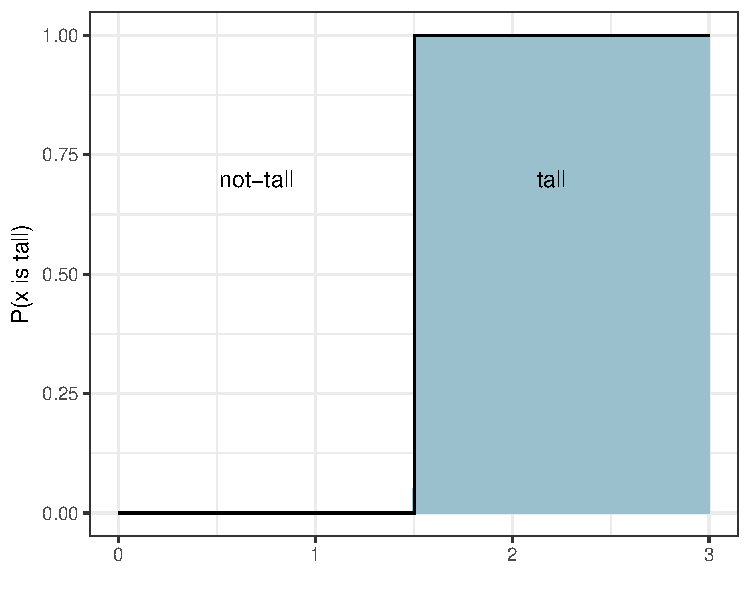
\includegraphics[width=0.5\textwidth]{cdf_crisp.pdf}
 	} 	
 	\subfloat[Vague meaning function with borderline cases, according to $P(\theta)$ in figure (d).\label{subfig:cdf-vague}]{
 	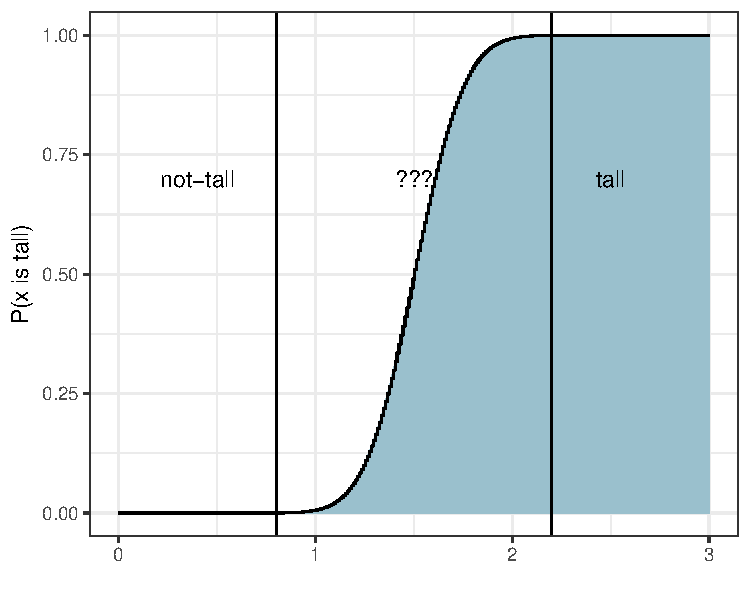
\includegraphics[width=0.5\textwidth]{cdf_vague.pdf}
 	}
 	\\
 	\subfloat[Exact belief about the value of $\theta$.\label{subfig:p-crisp}]{
    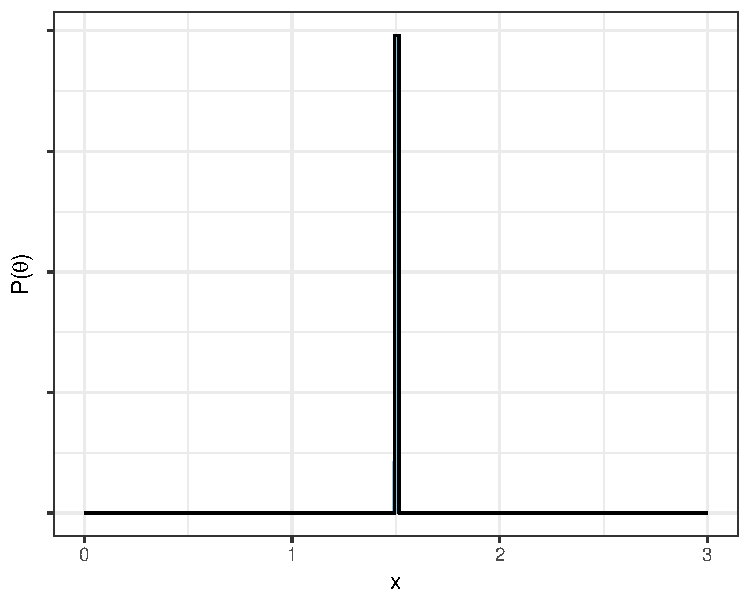
\includegraphics[width=0.5\textwidth]{p_crisp.pdf}
 	}
 	\subfloat[Uncertainty about the exact value of $\theta$.\label{subfig:p-vague}]{
    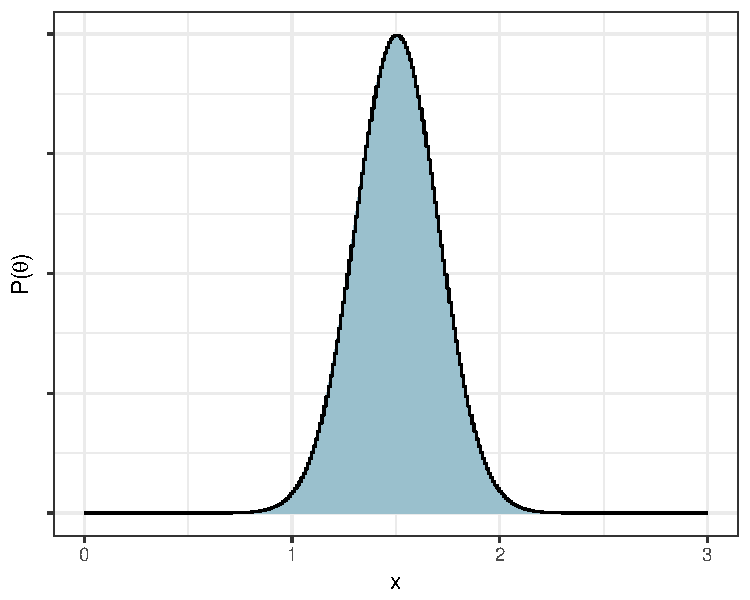
\includegraphics[width=0.5\textwidth]{p_vague.pdf}
 	}
 \caption{Schematic presentation of crisp and vague denotations.\\
 $P$(x is tall) = $\Phi(P(\theta)) \quad (\Phi =$ cumulative density function)}
 \label{figure:meaning}
\end{figure}
Another mode of use is a metalinguistic one: 
When you ask a basketball-player "What counts as \textit{tall} for you as a basketball-player?", and he answers "Phil, who is 2.12m, is tall", this means that his threshold for being tall is below Phil's height in this consideration. 
In this example, the use of the word \textit{tall} "eliminates [...] the possibility that the vague standard of absolute tallness might be greater than the maximal degree of [Phil's] height" \citep{barker2002dynamics}. Therefore, information about the underlying threshold $\theta_{tall}$ is provided, given the height of Marc.\\

As mentioned before, if the threshold is clear, as in "taller than exactly 1,80m", this would be called a crisp denotation instead of a vague one, although it is not referring to one specific world state. With this assumption, "vagueness" can be understood as uncertainty about the exact value of the threshold $\theta$.\\

What this uncertainty means for the semantics of gradable adjectives can be formalized as a probability distribution $P(\theta)$ over the possible values for $\theta$. In Figure \ref{subfig:p-crisp}, all probability mass lies on one point, there is no uncertainty about the value of the threshold. The meaning of the word \textit{tall} then is true (=1) for world states greater than $\theta$ and false (=0) for smaller world states. This "meaning function" is visualized in \ref{subfig:cdf-crisp} and is given by the cumulative density function ($\Phi$) of the the distribution $P(\theta)$. The resulting step function $P(x \textsf{is tall} \mid x) = \Phi(P(\theta))$ can be understood as a model of a crisp denotation. Fig. \ref{subfig:p-vague} shows a Gaussian distribution with mean $\mu$ and standard-deviation $\sigma$ over the possible values for $\theta$, indicating uncertainty about this value. Again, when looking at the cumulative distribution function of $P(\theta)$ in Fig. \ref{subfig:cdf-vague}, the behavior/meaning of a "vague" term is modeled well, in the sense that there are clear cases and borderline cases. It also feels intuitive that the degree to which an object counts as e.g. \textit{tall} increases with its size. This kind of formalization will later be used as an implementation of the semantics in a computer simulation.

\section{Computer simulations for language evolution}
When investigating language evolution or certain properties of language itself, it can be difficult for researchers to perform experiments to  gather data and evidence. It is impossible to change certain aspects of language in an experimental setup, because a person's language representation is deeply grounded within cognition. In many scientific fields, direct observation is not possible and therefore, analytic models and computer simulations might give evidence for developing theories.\\

For setting up a computational model about some property of language, it must be clear which language features are assumed and what features are to be examined. An undesirable direct link between some (global) mechanism in the simulation and the feature to be explained must be avoided. For truly exploring the effects of a certain property, the feature under interest needs to be somehow related to this property, rather than being determined by some (global) mechanism that cannot be observed clearly. Make sure to link an effect to the right cause.\\

Also, there is need for considering configurations that lead to the expected results, as well as configurations that lack the "desired" properties \citep{steels2006experiments}. So called "probabilistic models" are one way of accessing the actual implementation of cognitive processes based on probabilities and statistic inference mechanisms. In a probabilistic generative model there is a formal description about how states of the world are generated or how decisions are made. Often, basic assumptions about the world (e.g. the semantics of a vague term) and causality are stated in this description \citep{probmods2}.An application of probabilistic modeling/cognitive modeling is given in the next chapter, when introducing the Rational Speech Act model.\\

Probabilistic programming languages (PPL) provide a framework for setting up
probabilistic models and perform inference on these.
\textit{webPPL} \citep[by][]{dippl} is my choice of programming language in this work. It is embedded in JavaScript and provides a lot of functions associated with probability-computation, (Bayesian) inference algorithms such as MCMC techniques etc. It also integrates well into R, which I used for data analysis and plotting the results. 
\chapter{RSA - Model}
\label{chapter:rsa-model}
Human cognition allows us to pragmatically infer the meaning of utterances even beyond literal semantic meaning.
One common example is given by "scalar implicatures" as triggered by the word \textit{some} in "I ate some of your cookies". Taken literally, \textit{some} is compatible with \textit{all}, nevertheless we often infer that the speaker meant "some but not all". This is because we are assuming that the speaker wants to be informative. In a possible world where the speaker ate all cookies, he would have said "I ate all of your cookies", because this would give more information for the listener. By taking into account the speaker's alternative utterances and the use of them in various possible worlds, listeners implicitly entertain a model of the speaker's utterance choice. This model can be used for reasoning about the meaning of an utterance, which enables listeners "to make more informed interpretive choices than would be possible if they simply updated their information states with the information that the utterance's semantic interpretation is true." \citep{lassiter2017adjectival}\\

A formal model of language comprehension, that takes into account the listener's intuitive theory of how the speaker chooses words, is given through a "Rational Speech Act model" (RSA model), used by \cite{goodman2013knowledge}.
This chapter will introduce the main components of the RSA model as well as the underlying idea of probabilistic recursive reasoning. Afterwards, a new sort of extension to the RSA model is presented and evaluated.

\section{Main idea of RSA and Bayes' Theorem}
\begin{quote}
"RSA models language use as a recursive process in which
speakers and listeners reason about each other to enrich the literal semantics of their language.
This increases the efficiency and reliability of their communication compared to what more
purely literal agents can achieve." \citep{monroe2015learning}
\end{quote}
As mentioned in the citation above, the RSA model provides a description of an agent's language understanding and language production.
Numerous variations and applications of this model have been used for predicting phenomena like "scalar implicatures" or non-literal understanding of number words \citep[see][]{goodman2013knowledge, kao2014nonliteral}. By now, the RSA model has mostly been used to model language behavior by assuming a fixed set of utterances and their semantics. This set of semantics is given by a (hand-built) lexicon. Before introducing the concrete implementation of an agent's inference strategies, the following paragraph will give a brief explanation of \textbf{Bayes' Theorem}, which will be used in the description later.
Bayesian inference in general is introduced by \cite{lassiter2017adjectival}, 
therefore I will focus on the following theorem:
\begin{theorem}[Bayes' Theorem]
$P(B \mid A) \propto P(A \mid B) \cdot Pr(B)$
\end{theorem}
It provides a rather simple formula for calculating \textit{a-posteriori}-probabilities (the probability of hypothesis $B$ to be true, after seeing some event $A$). For this you need to know the conditional probability of $A$ being true, given hypothesis $B$, as well as the \textit{a-priori}-probability of $B$ being true (the probability of $B$ being true, without considering any further indications). Note that there is no equality sign. For equality, the right side of the formula must be derived by the marginal probability $P(A)$. While $P(A)$ is generally hard to compute, proportionality is assumed instead of equality ($A \propto B$ means that $A$ is directly proportional to $B$). This allows to omit the normalizing constant $P(A)$ and still obtain similar results. This inference technique is used for modeling the language behavior of an agent, as described in the following section.

\section{Inference strategies in RSA}
Consider a communication situation like the one described in section \ref{sec:egt}. A non-pragmatic "literal listener $L_0$" simply updates it's prior information state on the truth-value of an utterance $m$. $L_0$ infers a world state $w$ (e.g. the height of a person) after hearing a message $m$ (e.g. \textit{tall}), updating his prior information state $Pr(w)$ using an instance of Bayes Theorem. The formula is given in Eq.\ref{eq:L0-rsa} below.
\begin{equation}
\label{eq:L0-rsa}
P_{L0}(w \mid m) \propto \llbracket m \rrbracket^w \cdot Pr(w) 
\end{equation}
The "meaning-function" $\llbracket m \rrbracket^w$ takes on values between zero and one, representing the degree to which a message $m$ is true in world state $w$. Therefore it can also be formulated as $P(m $ is true $ \mid w)$.
"$Pr(w)$ specifies $L_1$'s background knowledge about answers to the QUD. For
example, if the QUD is 'How tall is Al?' and $L_1$ knows only that Al is an adult man,
then $Pr(w)$ is an estimate of the distribution of heights among adult men" \citep{lassiter2013context}. The presented model of a literal listener is used to model rational/informative speaker behavior as described in the following paragraph.\\

An informative speaker chooses an utterance $m$ from a finite set of alternatives $M$. The choice is made by reasoning about how a hypothetical literal listener $L_0$ would understand an utterance in the present circumstances.
In general, for capturing a speaker's motivation to be informative, the informative content for the listener is to be maximized. A false utterance will not provide any informative content and therefore is not likely to be chosen by a rational speaker. In order to model informative behavior mathematically, the utility $U$ of a message $m$ for the speaker $S_1$ is defined to be proportional to the informative content/informativity for the listener, who is reasoning about the true answer (the true world state) $w$.
The definition of informativity used here is given by \cite{lassiter2013context}:\begin{quote}
"Informativity is quantified as negative surprisal (positive log probability) of the true answer in the posterior, assuming that the utterance is true under the relevant parametrization."
\end{quote}
Negative surprisal is to be understood here as the amount of information that $L0$ would still not know about $w$, after hearing message $m$:
\begin{equation}
U_{S1}(m, w) = log(P_{L0}(w \mid m))
\end{equation}
After applying a soft-max choice rule to the utility function (which means that the probability of making a certain choice increases with its utility), the informative speaker model is obtained. The probability of choosing a certain utterance $m$, given an observed world state $w$, is given in Eq.\ref{eq:S1-rsa}.
The formula contains a "rationality parameter" $\alpha$ > 0. It determines how closely the stochastic choice approximates the deterministic utility-maximization i.e. the deviation from optimality. The effect of this parameter on the actual inference strategies is discussed later in this chapter. The notion of "recursive reasoning" is derived from the assumption that listeners and speakers maintain probabilistic models about each others behavior that drive pragmatic language use.
This idea of recursive reasoning is embedded in the formalization of the inference behavior of a pragmatic listener $L_1$. Messages are interpreted by reasoning about the speaker-model, which itself contains reasoning about a listener-model. This is done by taking into account what the speaker is likely to say, given a certain observation $w$ as well as the prior probability of $w$, as given in Eq.\ref{eq:L1-rsa}:
\begin{align}
\label{eq:S1-rsa}
P_{S_1}(m \mid w) &\propto exp(\alpha \cdot U_{S1}(m,w))\\
P_{L_1}(w \mid m) &\propto P_{S_1}(m \mid w) \cdot Pr(w)
\label{eq:L1-rsa}
\end{align}
The described models of pragmatic language understanding ($P_{L_1}$) and informative language use ($P_{S_1}$) will now be used for specifying language behavior of artificial agents. An innovative extension to the model is presented, that allows to take into account different underlying semantics.\\
The extended model will later be used for simulating a population of rational agents and their respective language use/understanding along Gricean lines. 
Chapter 5 examines which strategies/semantics are optimal, assuming that the agents behave according to the RSA model. This is a rather new application of the model.

\section{Agent types}
What properties define an agent in this scenario? An agent is fully described by its underlying \textit{type} $t$. A \textit{type} consists of three parameters:
$\mu, \sigma$ and $\alpha$. The following sections will describe the speaker and listener behavior as a mapping from their type $t$ to the respective inferences, according to the RSA model.\\

The parameters $\mu$ and $\sigma$ feed into a Gaussian distribution that represents the belief about the semantic threshold $\theta$, after which to use \textit{tall} (or \textit{short} likewise). Figure \ref{subfig:p-crisp} shows an exact belief about the value of $\theta$, with $P(\theta \mid \mu = 1.5, \sigma=0.001)$. This type would result in a crisp interpretation/a crisp meaning function, as in Fig.\ref{subfig:cdf-crisp}. On the other hand, a bigger $\sigma$ leads to a more vague interpretation/meaning function, see Fig.\ref{subfig:p-vague} (with $P(\theta \mid \mu=1.5, \sigma=0.2)$ and Fig.\ref{subfig:cdf-vague}.\\

Parameter $\alpha$ models an agent's "degree of rationality"/"optimality".
A more detailed explanation of the type's effect on the resulting inference strategies is given in the following sections, where the original formulas of the RSA model are extended by the type of an agent.

\section{Literal listener $L_0$}
%% L0 was displayed wrong because of discrete world Prior with 0.1-steps.
%% Set the discretization-steps to 0.00001, and the result looks as expected.
\begin{figure}[h]
 	\centering
 	\subfloat[L0-type: $\mu=1.5,\, \sigma=0.0001,\, \alpha=10$\label{subfig-1:L0_crisp}]{
 	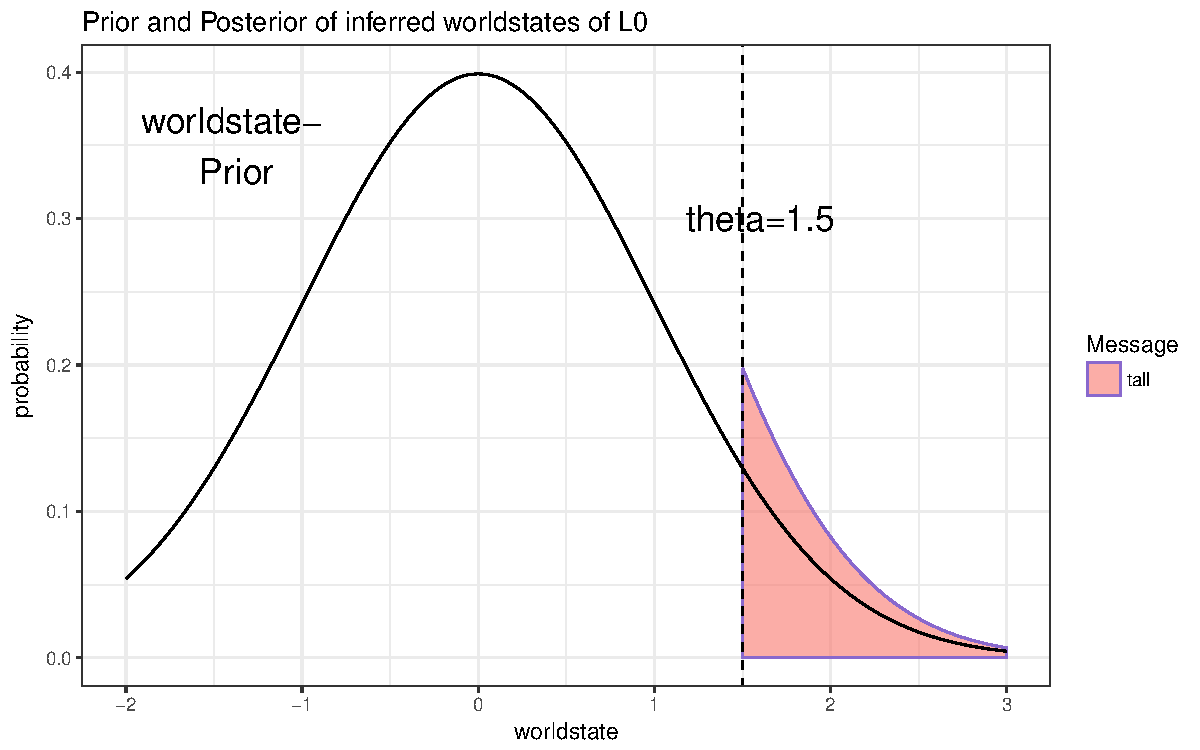
\includegraphics[width=0.5\textwidth]{L0-schematic-crisp.pdf}
 	} 	
 	\subfloat[L0-type: $\mu=1.5,\, \sigma=0.3,\, \alpha=10$\label{subfig-1:L0_vague}]{
 	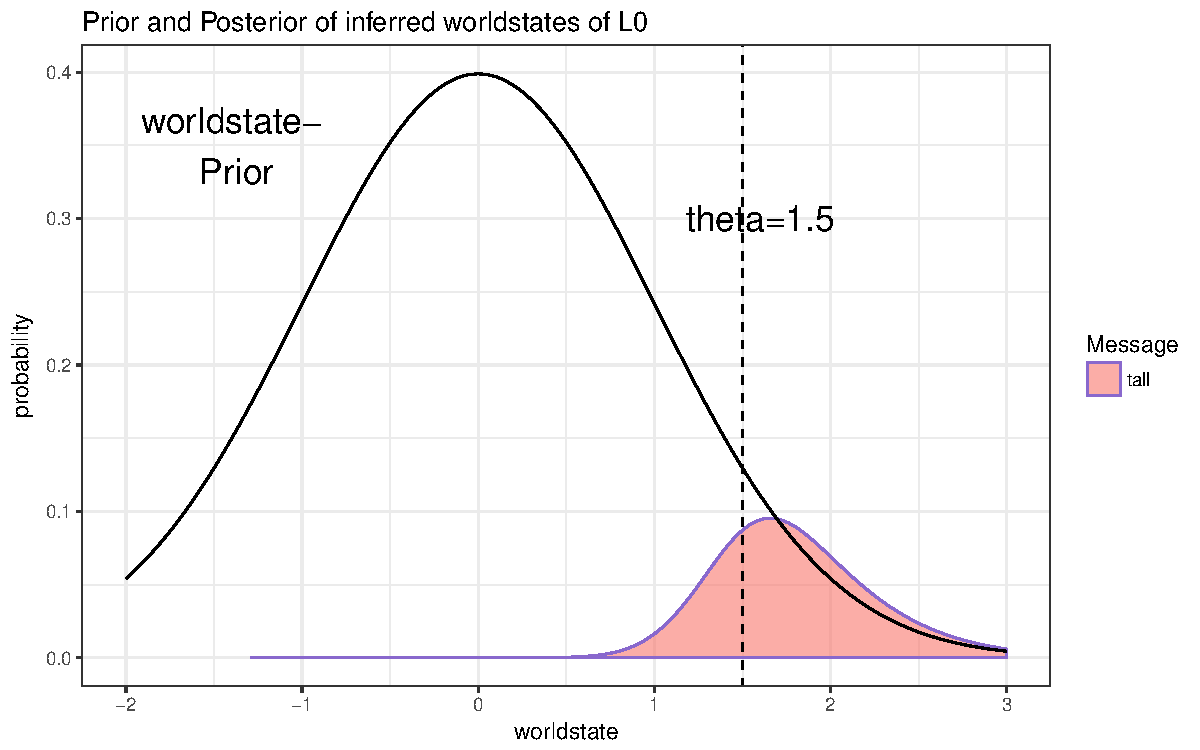
\includegraphics[width=0.5\textwidth]{L0-schematic-vague.pdf}
 	}
 \caption{Literal listener posteriors for a crisp and vague type.}
 \label{figure:L0-posterior}
\end{figure}
A literal listener is considered to interpret an utterance by its literal meaning. The interpretation results in a belief about the world state that was described by the speaker i.e. an answer to the current question under discussion. 
This might be e.g. the number of cookies eaten when your friend says he "ate some of the cookies" and is represented through a probability distribution over possible world states.
Another example for inference over world states can be the height of people, after hearing the sentence "Marc is tall".\\

By extending the original model by an agent's type $t = \big[ \mu, \sigma, \alpha\big]$, the resulting definition of the literal listener $L_0$ looks like this:
\begin{equation}
P_{L0}(w \mid m , \big[ \mu, \sigma, \alpha\big]) = \llbracket m \rrbracket^{w,\mu,\sigma} \cdot Pr(w) 
\end{equation}
A possible implementation of the meaning function $\llbracket m \rrbracket$ was given in section 2.3. The type-parameters $\mu$ and $\sigma$ model the distribution $P(\theta)$ and the literal meaning of an utterance $m$ under $w$ is derived by $P(\theta)$ in the following way:
\begin{equation}
\llbracket m \rrbracket^{w,\mu,\sigma} = P(m \, \textsf{is true} \mid w, \mu, \sigma) = \Phi(P(\theta \mid \mu, \sigma))(w)
\label{eq:meaning-func}
\end{equation}
This truth-functional meaning function is used by $L_0$. For the simulation in chapter \ref{chapter:simulation}, I will go further into detail on the implementation of the literal meaning function for the alternatives \{\textit{short}, \textit{not-short}, \textit{not-tall}, \textit{tall}\}, following Eq.\ref{eq:meaning-func}.\\

Using Bayesian inference and conditioning the prior information state on the truth of message $m$ results in a posterior probability distribution over possible world states, i.e. an interpretation of $m$. Different types result in different interpretations, as visualized in Figure \ref{figure:L0-posterior}, with the example $m = tall$. 
The strategy of $L_0$ is a mapping from its type to an interpretation of message $m$. 
Note, that $\alpha$ does not occur in the definition of the literal listener $L_0$, but it will be explained in the next section. 

\section{Informative Speaker $S_1$}
\begin{figure}[h]
 	\centering
 	\subfloat[S1-type: $\mu=1.5,\, \sigma=0.3,\, \alpha=1$\label{subfig-1:S1_naive}]{
 	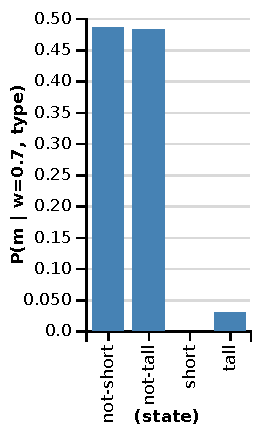
\includegraphics[width=0.35\textwidth]{S1-alpha1.pdf}
 	} 	
	\qquad \qquad
 	\subfloat[S1-type: $\mu=1.5,\, \sigma=0.3,\, \alpha=100$\label{subfig-1:S1_rational}]{
 	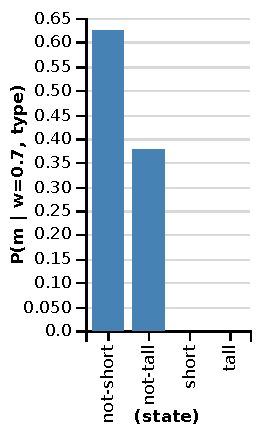
\includegraphics[width=0.35\textwidth]{S1-alpha100.pdf}
 	}
 \caption{Speaker choices of a naive and rational type, for $w=0.7$}
 \label{figure:S1-posterior}
\end{figure}
In this framework, the speaker is considered to select utterances that are informative relative to the current question under discussion. The choice of an utterance is made with respect to the alternatives and is now extended to be also dependent on type $t = \big[ \mu, \sigma, \alpha\big]$:
\begin{align}
P_{S1}(m \mid w, \big[ \mu, \sigma, \alpha\big]) &\propto exp(\alpha \cdot U_{S1}(m,w, \big[ \mu, \sigma, \alpha\big]))\\
U_{S1}(m, w, \big[ \mu, \sigma, \alpha\big]) &= log(P_{L0}(w \mid m, \big[ \mu, \sigma, \alpha\big]))
\end{align}
As mentioned before, one property of an agent's  strategy is its "degree of rationality", which is modeled through the parameter $\alpha$. $\alpha=0$ means, the choice of the message is made completely random, as a uniform draw from $M$. $\alpha=\infty$ means, the speaker is completely rational in the sense, that the choice truly optimizes the utility. This effect is visualized in Fig.\ref{figure:S1-posterior}. The message choices for describing the world state $w=0.7$ are shown, for a naive speaker (with $\alpha=1$) and a rational speaker (with $\alpha=100$). It can be seen that for a small $\alpha$, there is no clear preference for either of the messages. A more rational agent with a bigger $\alpha$ shows clearer preferences. This effect will get clearer when looking at the posteriors of $L_1$, in the next section.

\section{Pragmatic listener $L_1$}
\begin{figure}[h]
 	\centering
 	\subfloat[L1-type: $\mu=0.8,\, \sigma=0.01,\, \alpha=1$\label{subfig-1:L1_crisp_1}]{
 	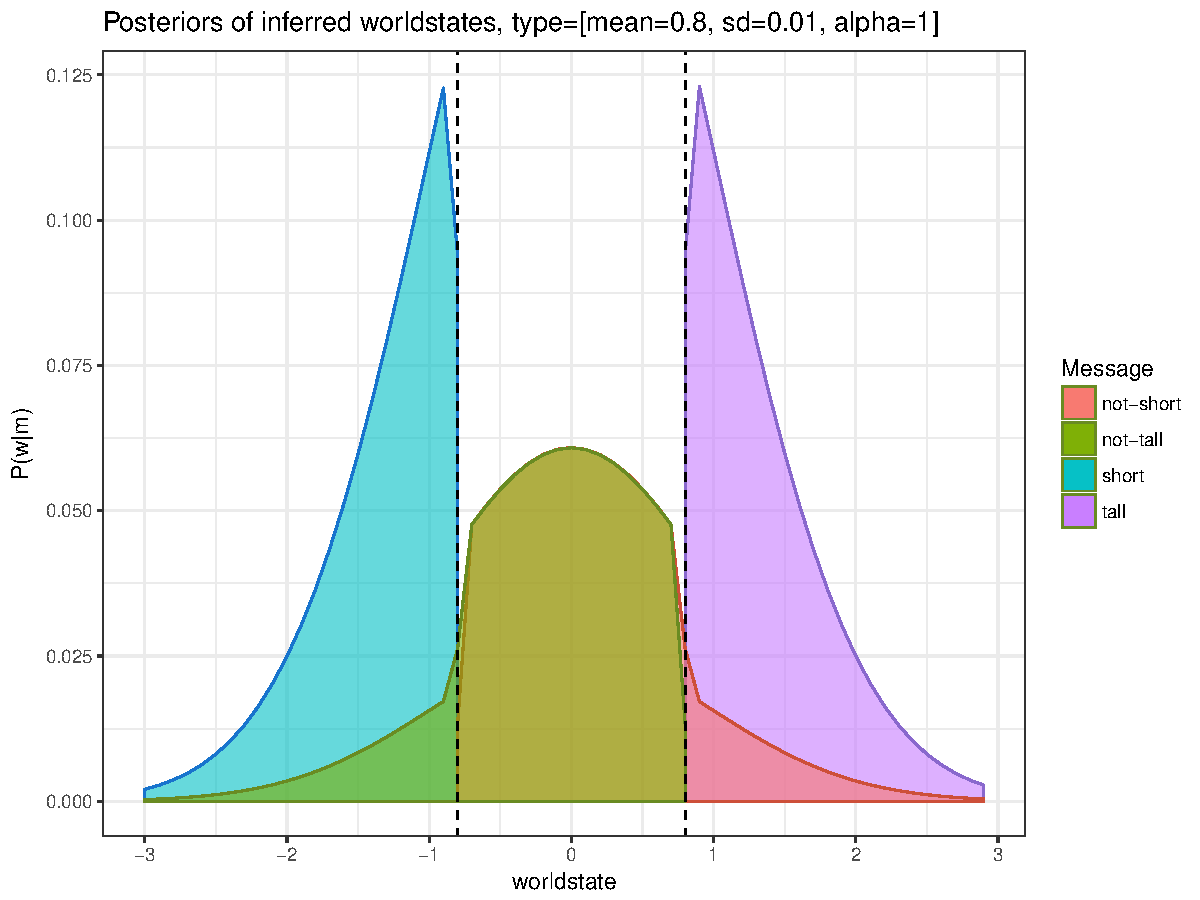
\includegraphics[width=0.5\textwidth]{L1_crisp_alpha=1.pdf}
 	} 	
 	\subfloat[L1-type:$\mu=0.8,\, \sigma=0.01,\, \alpha=50$\label{subfig-1:L1_crisp_50}]{
 	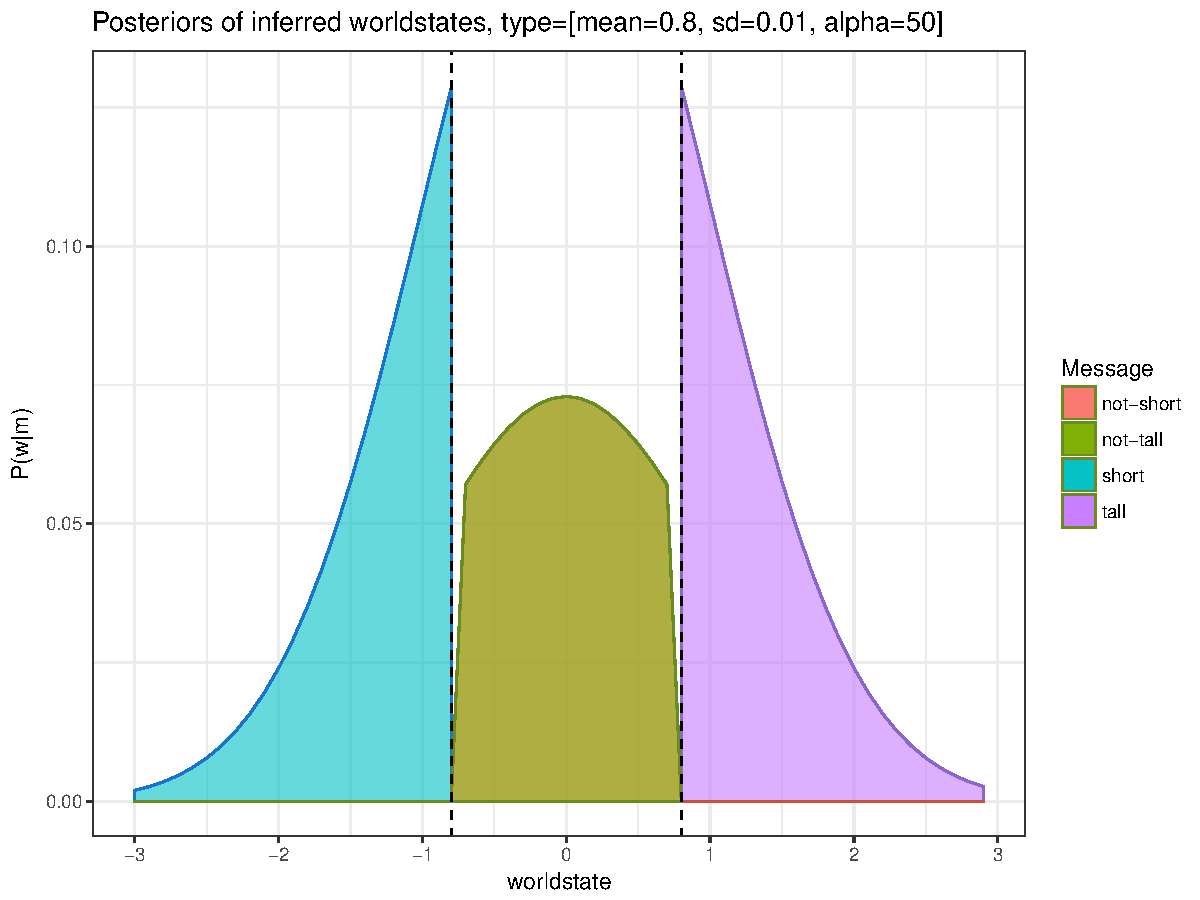
\includegraphics[width=0.5\textwidth]{L1_crisp_alpha=50.pdf}
 	}
 	\\
 	\subfloat[L1-type:$\mu=0.8,\, \sigma=0.5,\, \alpha=1$\label{subfig-1:L1_vague_1}]{
    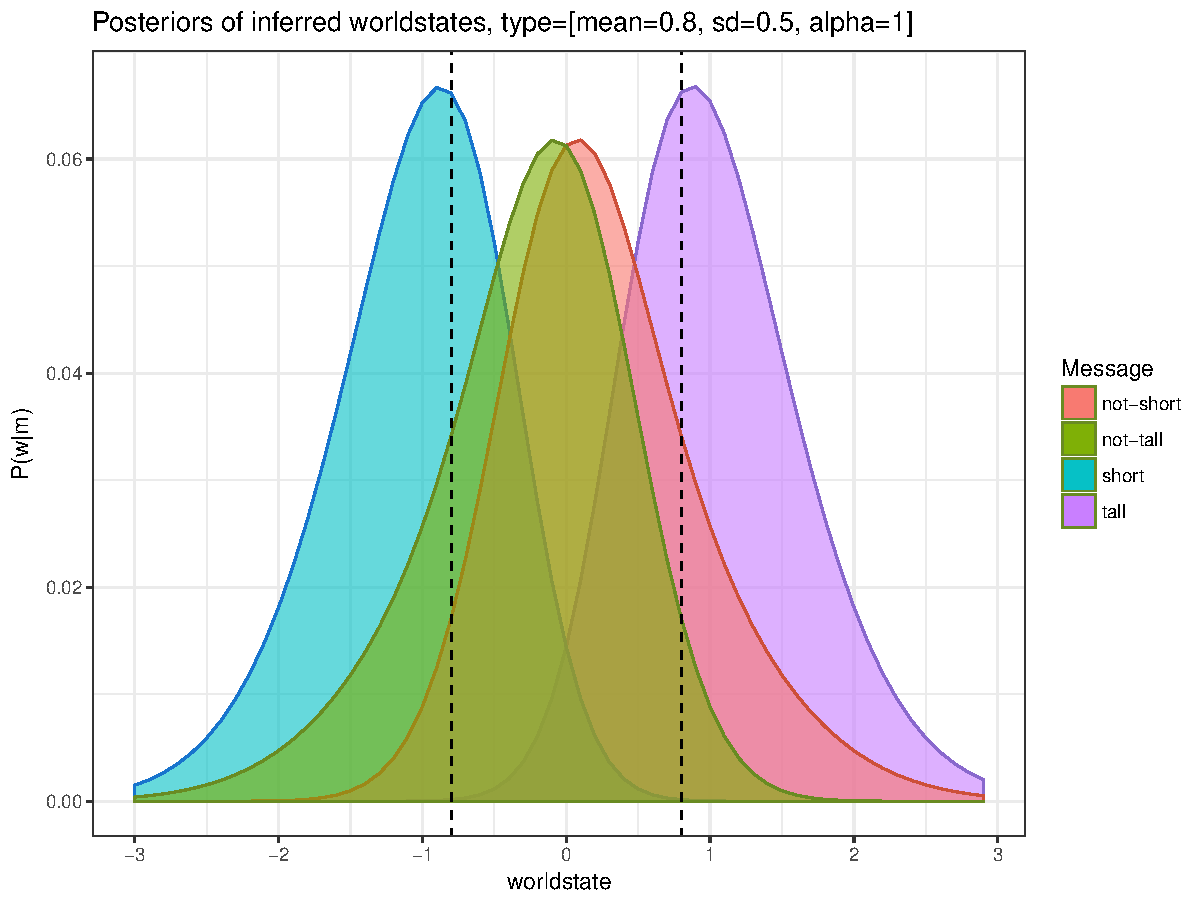
\includegraphics[width=0.5\textwidth]{L1_opt_alpha=1.pdf}
 	}
 	\subfloat[L1-type:$\mu=0.8,\, \sigma=0.5,\, \alpha=50$\label{subfig-1:L1_vague50}]{
    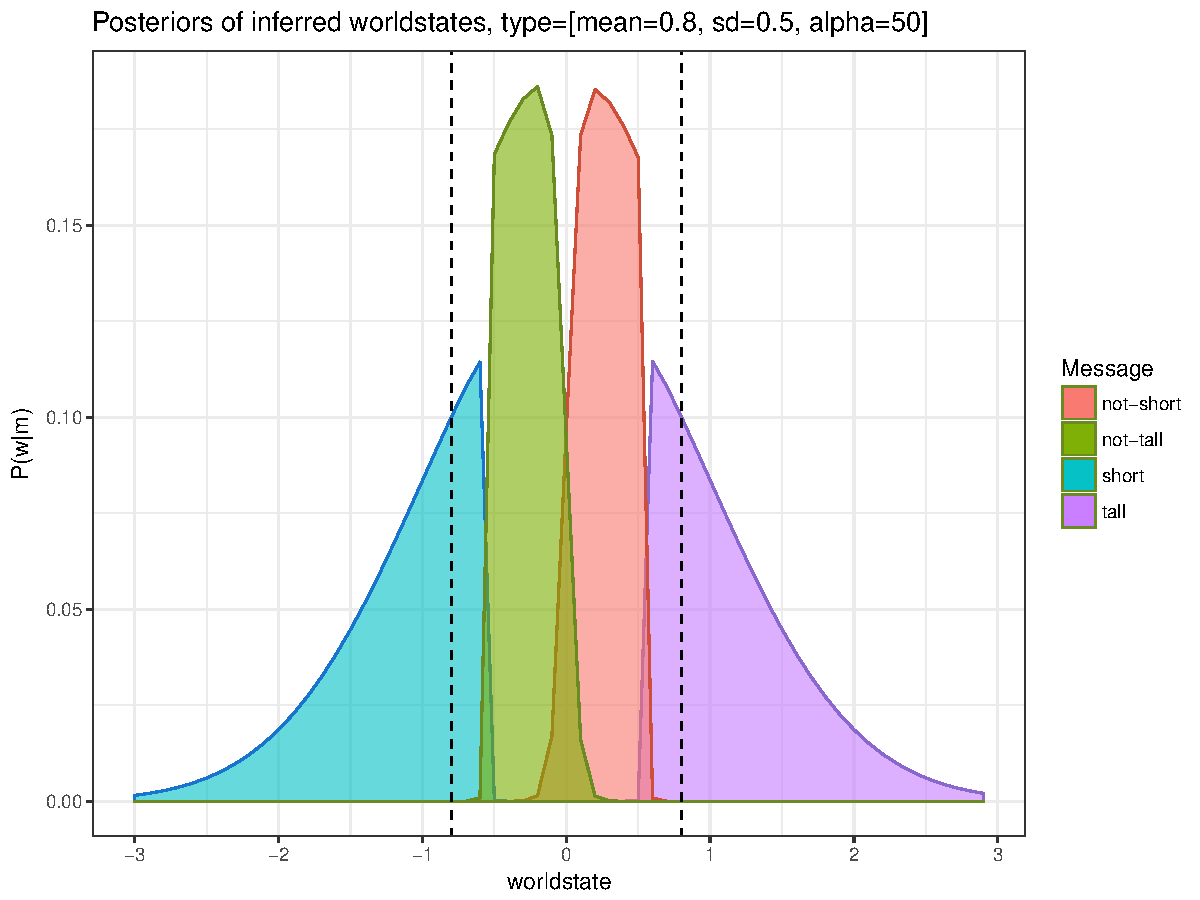
\includegraphics[width=0.5\textwidth]{L1_opt_alpha=50.pdf}
 	}
 \caption{Listener posteriors for different types}
 \label{figure:L1-posterior}
\end{figure}
The extension of $L_1$ is rather straightforward:
\begin{equation}
P_{L_1}(w \mid m, \big[ \mu, \sigma, \alpha\big]) \propto P_{S_1}(m \mid w, \big[ \mu, \sigma, \alpha\big]) \cdot Pr(w)
\end{equation}
Parameters $\mu$ and $\sigma$ are passed through to the level of $L_0$, where they are used for resolving the literal meaning of an utterance. Parameter $\alpha$ is passed trough to the level of $L_1$, where it determines the "optimality" of an agent's choice. Different posterior distributions for different listener types are presented in Figure \ref{figure:L1-posterior}. The effect of the parameters $\alpha$ and $\sigma$ on the resulting strategies is discussed below.\\

The effect of a small alpha ($\alpha=1$, Figures \ref{subfig-1:L1_crisp_1} and \ref{subfig-1:L1_vague_1}) can be found in the left column, a bigger alpha ($\alpha=50$, Figures \ref{subfig-1:L1_crisp_50} and \ref{subfig-1:L1_vague50}) in the right column. The first row shows a crisp listener strategy (type with $\mu=0.8$, $\sigma=0.01$ and $\alpha$ as described above), i.e. posterior probability distributions over inferred world states after hearing a certain utterance. The second row shows a vague listener type (type with $\mu=0.8$, $\sigma=0.5$ and $\alpha$ as described above). For the crisp type with $\sigma = 0.01$, the inferred meanings after the thresholds are quite clear, which is no surprise given the implemented semantics. What is more interesting, that in the area between the thresholds, it is completely unclear which interpretation choices will be made. The inferred probabilities over world states are very similar after hearing \textit{not-tall} or \textit{not-short}. This is also true for the naive vague type in Fig.\ref{subfig-1:L1_vague_1} with the difference that the inferred meaning of \textit{tall} and \textit{short} is very vague around the threshold.\\

Only for the rational vague strategy in Fig.\ref{subfig-1:L1_vague_1} we can observe clear and separate preferences over world states after hearing different messages. The state space has been partitioned into categories. \textit{Tall} is roughly interpreted as "taller than $\theta$", analogous to the meaning of \textit{short}. Being \textit{not-short} means "slightly taller than the norm" and \textit{not-tall} means "slightly smaller than the norm".
The ordering of the utterances' meaning is similar to the results of \cite{tesslernot}.
Figure \ref{figure:L1-posterior} nicely displays that the rational use of vague terms leads to a better understanding of the respective logical negations, while a rational crisp strategy lacks this feature.

\chapter{Simulation}
\label{chapter:simulation}

After introducing the general underlying ideas and topics associated with the issue of this work, I will now explain the simulation, which is the core topic of this work and go further into detail. 
\cite{lipman2009language} argued "that we cannot explain the prevalence of vague terms in
natural language without a model of bounded rationality which is significantly different from anything in the existing literature". I will argue with the results of the simulation, that the prevalence of vague terms can be explained with the RSA model, which is a model of bounded rationality.
The human ability of recursive reasoning about the mind state of the communication partner might enable us to understand vague terms and infer correct world states after hearing them, in order to communicate efficiently.

\section{General assumptions and procedure}
A communication situation which is to be modeled here was already introduced in chapter 2, but I will again shortly recap the procedure of the sender-receiver-game:\\

There are two players/agents, a speaker $S$ and a listener $L$. $S$ observes a world state $w$, randomly drawn from a distribution function $Pr(w)$ (= world prior). In this case, $w$ is to be interpreted as the height of a person. Then, $S$ chooses a message $m$ from a set of alternatives $M$, to describe the observed $w$ to $L$, who cannot observe $w$ directly. Dependent on the observed message $m$, $L$ chooses an action $a$, which in this case is simply guessing the intended world state $w$. The probability, that listener $L$ infers the correct height is calculated for computing an "expected utility (EU)" value (more on EU in section \ref{sec:EU}). This serves as a measure of communicative success and is later used for evaluating the simulation results, in an examination of evolutionary stable strategies. A schematic figure of a communication situation is given in Fig.\ref{figure:procedure}.\\

Each agent is of a certain \textit{type}. These types differ in their belief about the actual semantics of a gradable adjective like \textit{tall}, more specifically in their belief about the underlying threshold, after which to use \textit{tall} (e.g. crisp vs. vague threshold). The next section should clarify the actual semantics of the possible utterances by showing an implementation of a lexicon that uses the meaning function defined in chapter 3. After that, I will make further assumptions about the world prior distribution from which the world states for the speaker's observation are drawn. At the end of this chapter, the actual simulation is presented and explained, including the quantitative measure of communicative success (EU).
\begin{figure}
 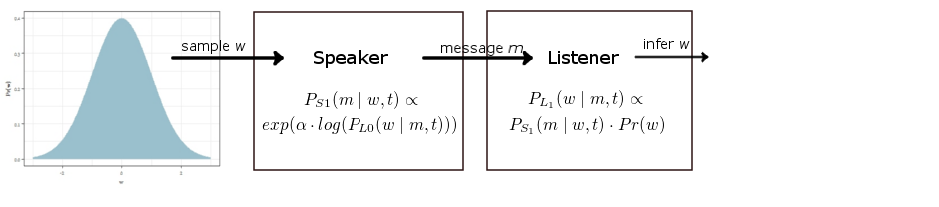
\includegraphics[scale=0.7]{procedure.png}
 \caption{Schematic presentation of a communication situation.}
 \label{figure:procedure}
\end{figure}
\section{Vague meaning in the lexicon}
How is a vague word like \textit{tall} to be interpreted? How can we quantitatively capture the vagueness in a semantic description in a lexicon? As introduced in chapter \ref{chapter:rsa-model}, I implemented the meaning as a degree to which an utterance is true, given the utterance and the \textit{type} of an agent, as a function over world states.\\

A "truth-function", for each possible utterance has to be implemented, in order to form a lexicon that serves as a rudimentary basis for language understanding and language use. The message set of alternatives considered here is $M = \{$\textit{short}, \textit{tall}, \textit{not-short}, \textit{not-tall}$\}$. Lexical antonyms like \textit{short} and \textit{tall} are treated differently than the respective logical negations \textit{not-short} and \textit{not-tall}. The behaviour of negated vague terms is not trivial, but has been empirically studied and quantitatively modeled by \cite{tesslernot}. Similar results can be replicated in this simulation, with respect to the use and understanding of the negation of vague terms and their antonyms.\\

One possibility for expressing meaning would be to consider different thresholds for \textit{tall} and \textit{short} as well as the interpretation of "not" as logical negation. In the following description, $w$ is some world state, i.e. a height value:
\begin{align*}
\text{"tall"} \rightarrow& \,\, w > \theta_{tall}\\ 
\text{"not-tall"} \rightarrow& \, \neg (w > \theta_{tall})\\
\text{"short"} \rightarrow& \,\, w < \theta_{short}\\
\text{"not-short"} \rightarrow& \, \neg (w < \theta_{short})\\
\end{align*}
Such an implementation of a meaning function maps a world state to either true or false (one or zero), like in Figure \ref{subfig:cdf-crisp}. For adding vagueness to the semantics, the threshold $\theta_{tall}$ is not given by a crisp number, but a Gaussian probability distribution over possible values for $\theta$. Language use changes over time, so it seems more natural to assume that the same world state might lead to different message choices of a speaker at different points in time, due to vague semantics. It also seems natural to assume that the degree to which the word \textit{tall} is true should increase gradually with increasing height $w$. This behavior is modeled well by a cumulative distribution function $\Phi$ over the prior expectation about $\theta$, as introduced in chapter \ref{chapter:rsa-model}. The concrete semantics for the utterances \textit{tall} and its negation are given below. The semantics for \textit{short} and its negation are analogous.
\begin{align*}
\llbracket \textsf{"tall"} \rrbracket^{w, \mu,\sigma} &= \Phi(P(\theta_{tall} \mid \mu, \sigma))(w)\\
\llbracket \textsf{"not-tall"}  \rrbracket^{w, \mu,\sigma} &= 1 - \Phi(P(\theta_{tall} \mid \mu, \sigma))(w)
\end{align*}
Little uncertainty about the value of the threshold is described by a small value for $\sigma$ in the threshold prior, resulting in a crisp meaning, while a bigger $\sigma$ will lead to a more vague interpretation. A visualization of such vague literal semantics can be viewed in Figure \ref{figure:litsemantics}.
As a natural consequence of this degree semantics, borderline cases are modeled correctly in the sense that it is not deterministic whether \textit{tall} is true or not for a certain $w$, but it is true to a certain degree.
\begin{figure}
 \centering
 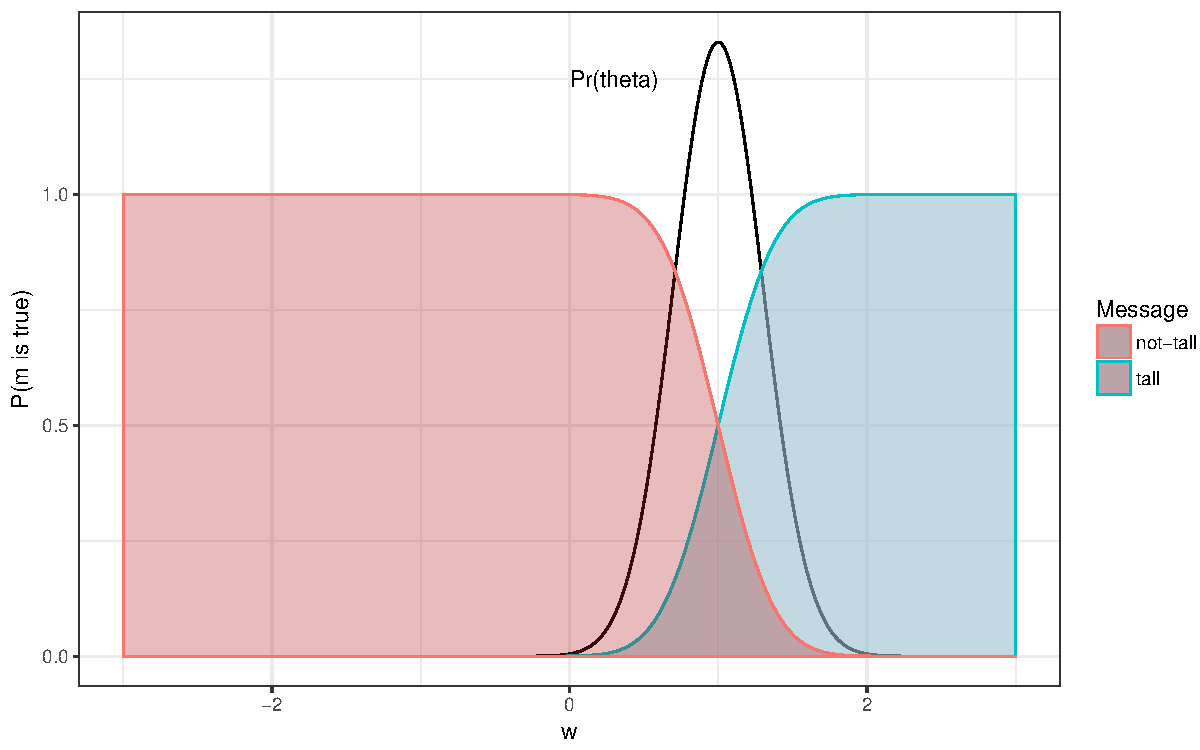
\includegraphics[scale=0.6]{lit_tall_vague.pdf}
 \caption{Literal vague meaning of \textit{tall} and \textit{not-tall}. The distributions for \textit{short} and \textit{not-short} look similar.}
 \label{figure:litsemantics}
\end{figure}

\section{World prior}

The chosen world prior distribution $Pr(w)$ of heights is a standard normal distribution with mean $\mu = 0$ and $\sigma = 1$. With this normalized choice, it is possible for interpretation to move this distribution to any scale of interest, like e.g. size of people, measured in m. 
It allows very general interpretations and brings the advantage of not having to specify a scale that is relevant, i.e. a comparison class.  It seems natural in the present model to capture the effect of a comparison class as an effect of the world prior choice. While comparison class inferences has been studied in other works, I will keep this factor standardized in this simulation.\\

Gradable adjectives seem to be interpreted in a "norm-related" way (Fara 2000), so that \textit{tall} would mean "taller than the norm", while the norm is dependent on a comparison class. This allows for symmetric behaviour of the thresholds for \textit{short} and \textit{tall}, because \textit{short} would also mean "shorter than the norm". It is considered that a deviation from the norm in the positive direction that counts as \textit{tall}, is the same deviation in the negative direction for counting as \textit{short}. From this assumption follows $\theta_{short} = -\theta_{tall}$.

\section{Goal of simulation}

An agent's type comprises a certain semantics. I want to investigate which semantics is optimal if agents behave rationally, according to the RSA model.
For measuring communicative success of two agent types, the probability that the speaker might choose a specific message $m$ for a specific world state $w$ is calculated, as well as the probability that the listener does "understand" this utterance, in the sense that the inferred world state equals $w$.\\

In the simulation, the "conversations" are simulated on all possible world states as well as all possible utterances. The overall expected utility (EU) is calculated for a given speaker- and listener type (more on the EU in the next section).
This calculation is performed on all possible pairs of all possible types of agents, to investigate which agent strategies perform well and which do not. 

\section{Expected Utility}
\label{sec:EU}
The expected utility (EU) of two agent types $t_1$ and $t_2$ quantifies the communicative success of these two agents playing the sender-receiver game repeatedly. $t_1$ and $t_2$ are considered to be the speaker and listener at half of the time respectively. To obtain $EU(t_1, t_2)$, I take into account each possible state $w$ as well as each possible utterance the speaker could make to describe the respective state. The EU of two agents is the probability that speaker $S_1$ would choose message $m$ and listener $L_1$ would infer the right world state $w$ after seeing $m$. This is summed over all possible world states and all possible messages, weighted with their prior probabilities. The message prior is uniformly distributed, therefore this term is omitted in the following formula:
\begin{align}
EU(t_1, t_2) = \sum \limits_{w} \sum \limits_{m} 0.5 \cdot \big[ &P_{S_1}(m\,|\,w ,\, t_1) \cdot P_{L_1}(w \mid m ,\, t_2) \cdot Pr(w) + \\
&P_{S_1}(m \mid w ,\, t_2) \cdot P_{L_1}(w \mid m ,\, t_1) \cdot Pr(w) \big] \nonumber
\end{align}
The simulation consists of an EU-computation for all possible agent pairs, for examining the effectiveness of different strategies/semantics. To evaluate which strategies perform best, I search for evolutionary stable strategies (ESS, this concept has been introduced in chapter \ref{chapter:vagueness-pragmatics}). Which agent types are used in the simulation is presented in the next section.

\section{Simulation set-up}

In the simulation, the types are combined from the following parameter spaces:
\begin{align*}
\mu &\sim \{ 0, 0.1, 0.2, ... , 2.0 \} \\
\sigma &\sim \{ 0.001, 0.1, 0.2, ... , 2.0 \} \\
\alpha &\sim \{ 1, 5, 10, 50, 100 \}
\end{align*}
All of these possible parameters are combined into a set of 2000 possible agent types in total, consisting of all possible combinations of the parameters $\mu$, $\sigma$ and $\alpha$. The set of $\mu$'s and $\sigma$'s could be chosen according to a comparison class, if this is desired. The results would look quantitatively different but qualitatively the same.
Example types would look like this: $t_1=[\mu=1.2, \sigma = 0.4, \alpha=5]$, $t_2=[\mu = 0.8, \sigma = 0.1, \alpha=50]$. A visualization of possible listener strategies is given in Fig.\ref{figure:L1-posterior}. It shows probability distributions over 
% message choices, $P(m | w, type)$ on the speaker side or 
interpretation choices, $P(w \mid m, type)$ on the listener side. In the following chapter the results of the simulation are presented, i.e. the EU-values for any agent pair as well as ESS. 
\chapter{Simulation Results}
\label{chapter:simulation-results}

In the simulation, in total 2000 different agent types (different triples of the type [$\mu$, $\sigma$, $\alpha$]) are present in the population. Every single of these 2000 agents got to communicate with every other agent. This makes in total $2000 \cdot 2000 = 4000000$ EU computations between different types of agents. In the following section, the expected utility data will be presented, described and interpreted.

\section{EU results}
\label{sec:eu-results}
Because of the amount of data points that are to be displayed, I chose a heatmap visualization for the EU results. Different types/parameters of interest are mapped on rows and columns of a two-dimensional matrix. Each cell in this matrix contains an EU score of $type_i$ vs. $type_j$.
The cells are colored depending on the EU score, with blue indicating low values, white for medium values and red indicating high values. An exact color-value-mapping can be found on the top left side of each plot.
To visually inspect the main effects of the three parameters that define an agent type ($\mu$, $\sigma$, $\alpha$) on the EU score, I marginalized out each parameter respectively. In Figure \ref{figure:alpha_marg}, a heatmap visualization is presented for the effect of the parameter $\alpha$.
\begin{figure}[h]
 \centering
 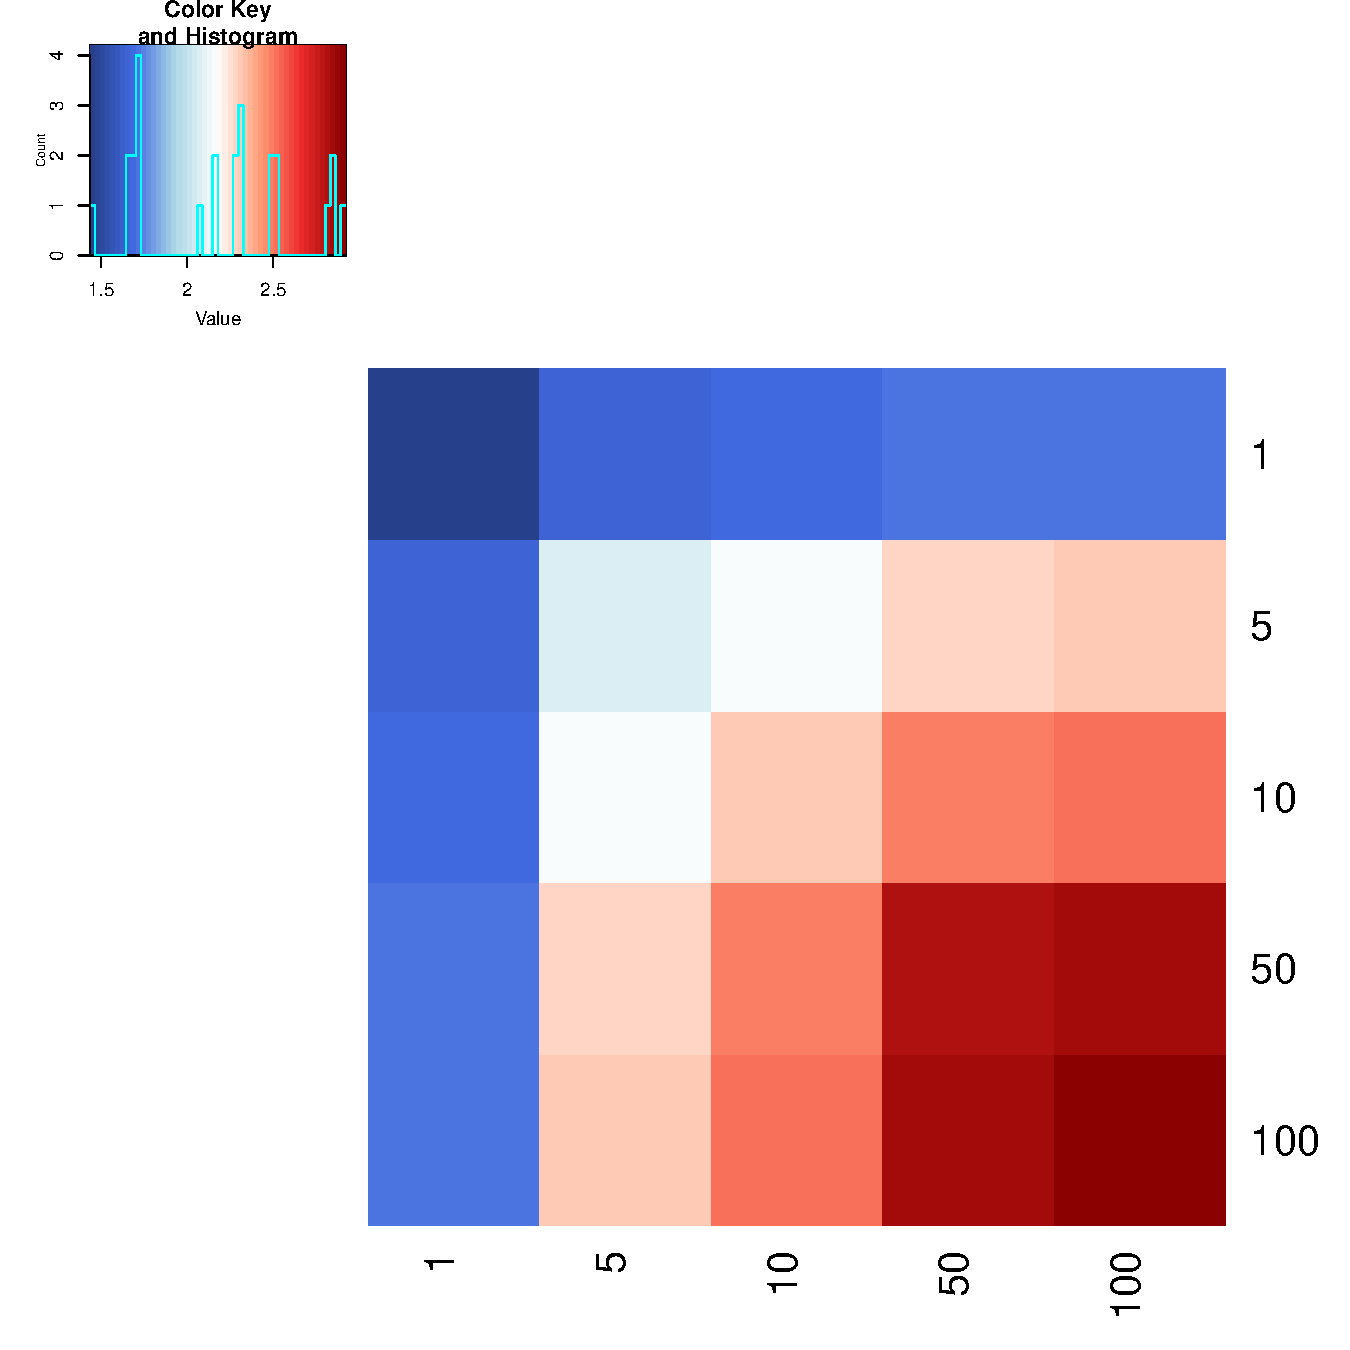
\includegraphics[width=0.7\textwidth]{alpha_marg.pdf}
 \caption{Effect of type parameter $\alpha$ on EU scores.}
 \label{figure:alpha_marg}
\end{figure}
On the x and y axis the possible alpha values are listed (1, 5, 10, 50, 100), in increasing order from left to right and top to bottom. One cell is an EU score of $type_i$ vs $type_j$. E.g. the top right cell contains the mean EU score that is obtained when a type with $\alpha=1$ plays with a type with $\alpha=100$ (that is the mean EU value of all types that have any possible $\mu$ and $\sigma$ values combined with this alpha).\\

The top row and left column (where $\alpha = 1$ on sender- and receiver side) contain low EU scores, this means that the overall success of irrational agents is rather low. In contrast, when looking at the bottom right cell, which contains the EU value of two maximally rational agents, the overall maximum score is obtained.
In conclusion, the EU scores increase with increasing alpha (top left cell: $\alpha=1$ vs. $\alpha=1$, bottom right cell: $\alpha=100$ vs. $\alpha=100$). This is because informative message choices on the speaker side and pragmatic inference methods on the listener side result in higher communicative success than more random choices. 
\begin{figure}[h]
 \centering
 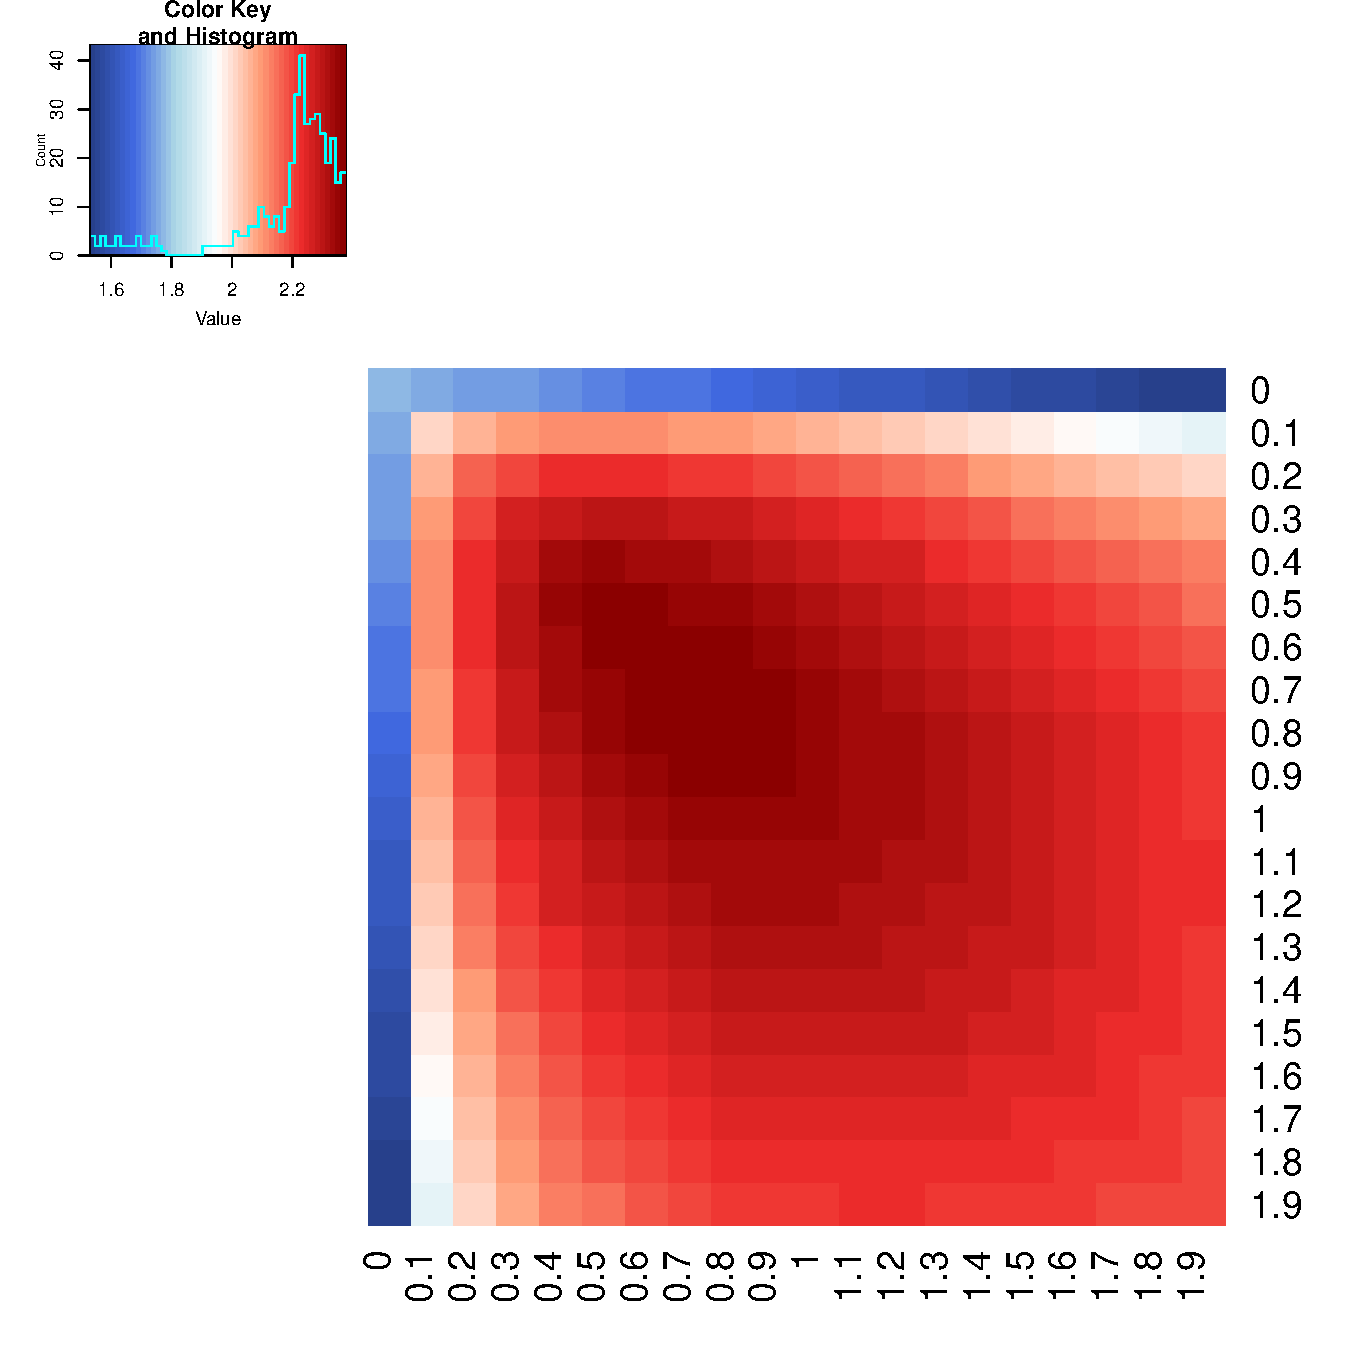
\includegraphics[width=0.7\textwidth]{mean_marg.pdf}
 \caption{Effect of type parameter $\mu$ on EU scores.}
 \label{figure:mean_marg}
\end{figure}
Figure \ref{figure:mean_marg} shows a heatmap plot for the effect of the $Pr(\theta)$ distribution parameter $\mu$. 
Again, all possible $\mu$'s (0, 0.1, 0.2, ..., 1.9) are listed on the axes in an increasing order from left to right and top to bottom. Again, one cell is a mean EU score that is obtained when types with $\mu_i$ play with types with $\mu_j$.
While low values like 0 or 0.1 generally lead to low EU scores (top row and left column), the highest scores can be obtained when both agents have a belief about the threshold with a $\mu$ between 0.5 and 0.9 (indicated by the dark red spot in the middle). This is because very weak interpretations, i.e. low threshold values, will mean that \textit{tall} is true for almost all world states, which is not informative. A very high threshold value is dispreferred because it restricts \textit{tall} to be true for just a few world states that are very likely to be false \textit{a priori}. It seems natural that rather medium values for $\mu_{\theta}$, that capture the meaning of \textit{tall} loosely as \textit{taller than average}, lead to the highest EU scores.\\

The effect of $\sigma$ is presented in Fig.\ref{figure:sigma_marg}. The ordering of possible $\sigma$'s (0.001, 0.1, 0.2, ... 1.9) is similar to the other two plots, increasing from top to bottom and left to right. The effect of $\sigma$ is particularly interesting, as it reflects the effect of "vagueness" in the literal meaning of e.g. \textit{tall} on the communicative success of agents using such a vague interpretation. For small $\sigma$'s, i.e. a crisp interpretation of the literal meaning of gradable adjectives, low EU scores are obtained, which is indicated by the blue rows and columns on the top and left edge of the heatmap.\\

The highest EU scores are obtained if both agents are of a type with $\sigma$ around 0.6 or 0.7. This indicates that a rather vague interpretation of the literal semantics leads to higher communicative success. The EU scores are maximal if the agent's vague beliefs about the semantics do not differ a lot from each other. Extreme discrepancies between beliefs, like e.g. $type_i$ with $\sigma_i = 0.1$ vs. $type_j$ with $\sigma_j = 1.8$ result in low EU scores, as in the upper right corner.
\begin{figure}[h]
 \centering
 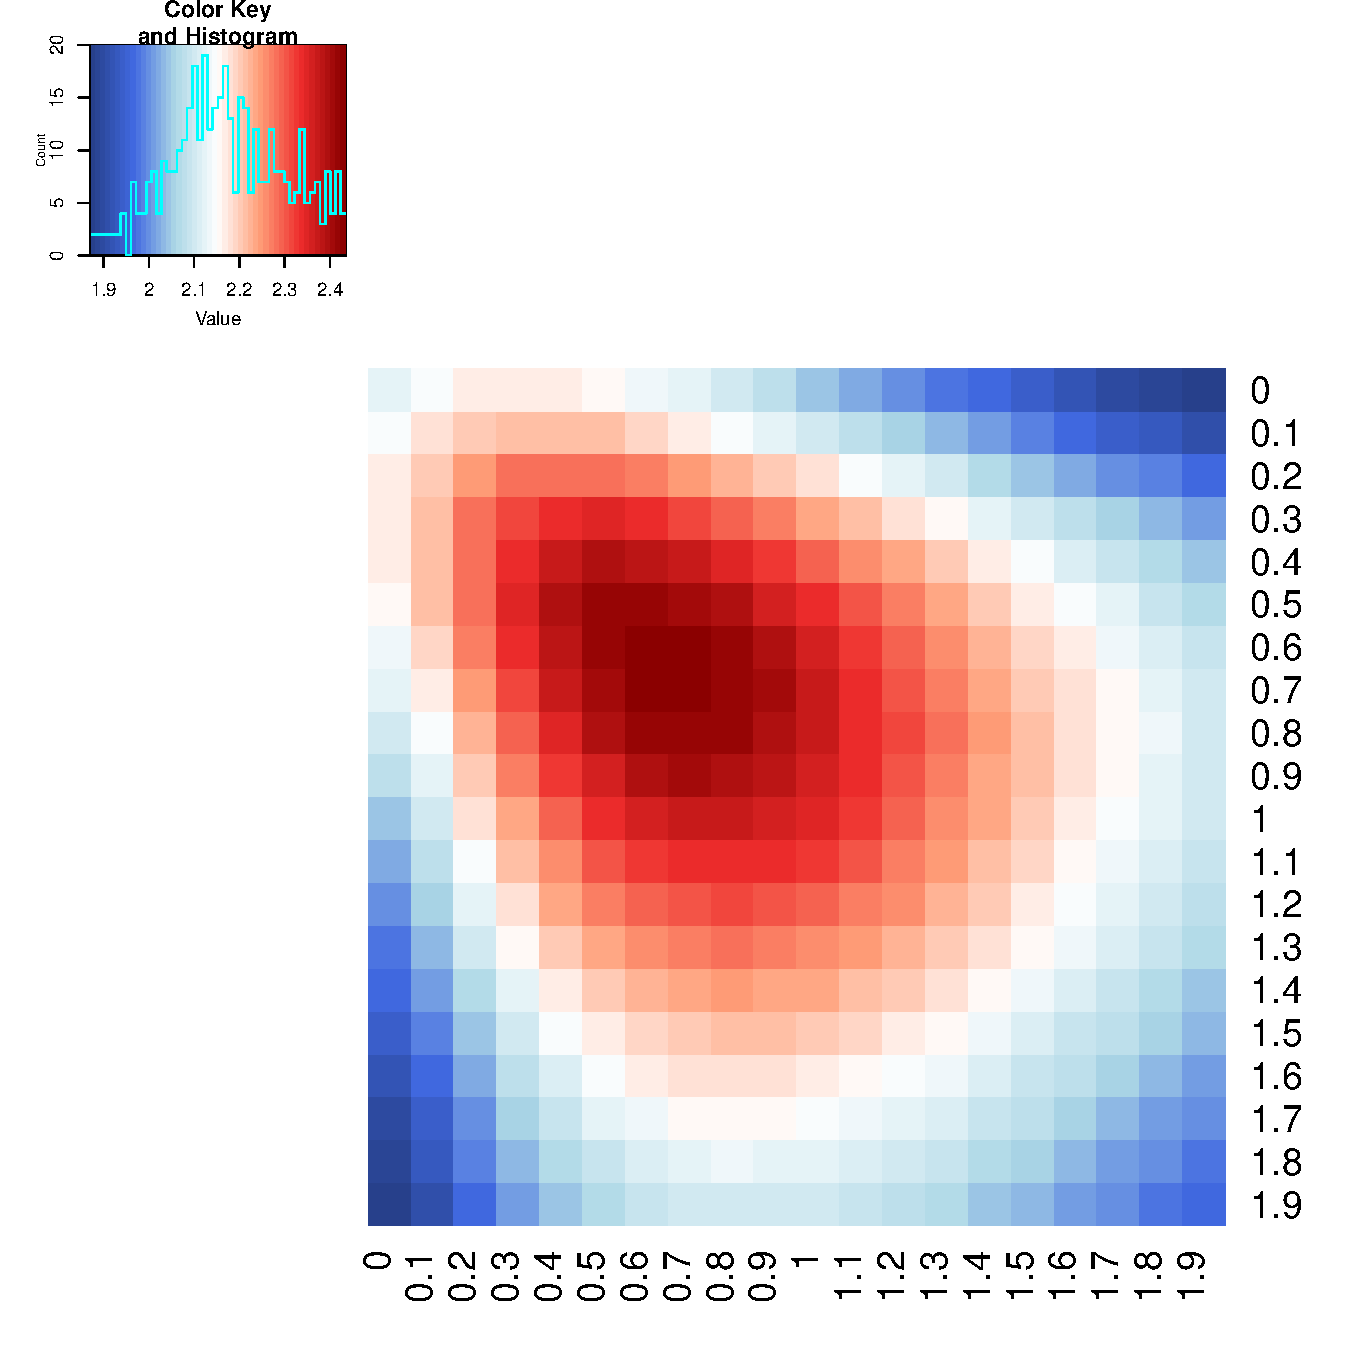
\includegraphics[width=0.7\textwidth]{sigma_marg.pdf}
 \caption{Effect of type parameter $\sigma$ on EU scores.}
 \label{figure:sigma_marg}
\end{figure}
These results could give evidence to one reason why vague terms, i.e. terms with vagueness in the literal meaning, are still prevalent in today's natural language understanding. A fairly vague interpretation of a word like \textit{tall} seems to be more successful in measures of "communicative success", than a crisp interpretation or a completely vague interpretation that is ambiguous.\\

Another very interesting effect is given through an interaction effect between the factors $\alpha$ and $\sigma$, i.e. rationality and vagueness, as displayed in Figure \ref{figure:sigma-marg-alpha}.
Three heatmaps of the effect of $\sigma$ are shown, while only agents with a fixed $\alpha$ value are considered in the calculation of the displayed mean EU values. The left figure shows the effect of $\sigma$ for agents with a low degree of rationality $\alpha = 1$. Agents with $\alpha = 10$ are considered in the middle plot and the effect of $\sigma$ for more rational agents, i.e. $\alpha = 50$ is shown in the right plot.\\

For a low $\alpha$ value (Fig.\ref{subfig:sigma_marg_alpha1}), the highest EU scores can be obtained for $\sigma$ being really small (0 or 0.1), i.e. for a crisp semantics of the messages.  Irrational agents seem not to be able to make use of vagueness in the interpretation of an utterance. For higher $\sigma$ values, i.e. more vague interpretations, low EU values are received.
In contrast, for more rational agents with $\alpha=50$, low EU scores are obtained for small $\sigma$'s. In this case, the $\sigma$ value that leads to the highest EU scores lies between 0.9 and 1.1, if both agents are rational and share the same vague belief about the meaning. In total, the optimal $\sigma$ seems to increase with increasing $\alpha$. This tendency can be seen by comparing the three heatmap plots in Figure \ref{figure:sigma-marg-alpha}.
A possible interpretation is the following:\\

An irrational agent would prefer crisp interpretations of messages, because they are unambiguous and do not need complex inference techniques for guessing the right interpretation. A rational agent can make use of a certain vagueness level and obtain overall higher EU scores due to the pragmatic language understanding and recursive reasoning. If agents differ strongly in their type, the communicative success is worse than if they would share the same belief about the interpretation, which seems quite intuitive.
\begin{figure}
 	\centering
 	\subfloat[][Effect of $\sigma$ on EU-scores 
 	
 	with $\alpha=1$.\label{subfig:sigma_marg_alpha1}]{
 	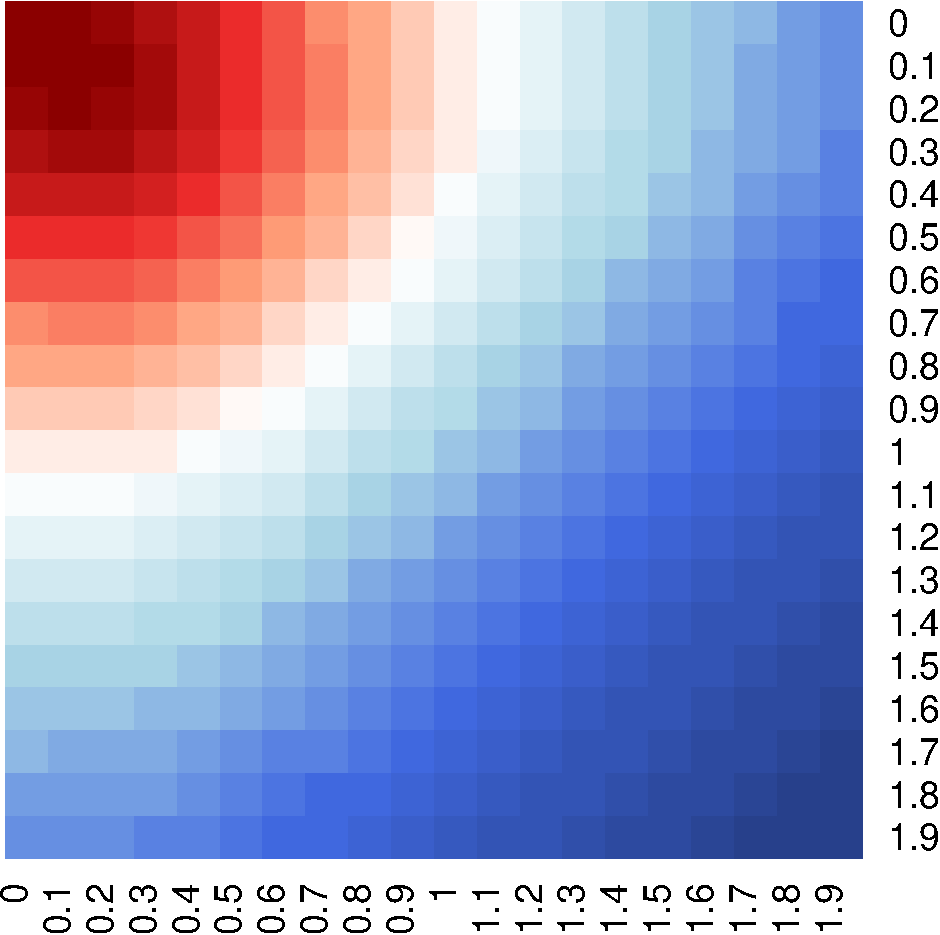
\includegraphics[width=0.33\textwidth]{sigma_marg_alpha=1.pdf}
 	} 	
 	\subfloat[][Effect of $\sigma$ on EU-scores 
 	
 	with $\alpha=10$.\label{subfig:sigma_marg_alpha10}]{
 	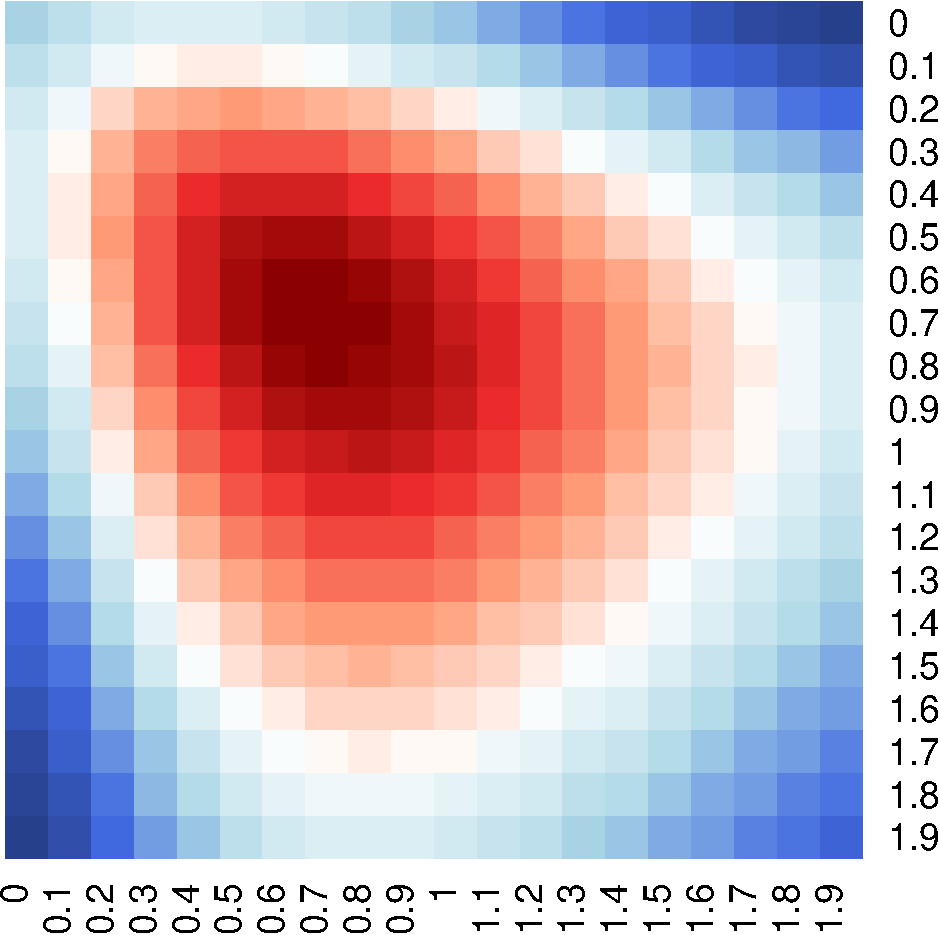
\includegraphics[width=0.33\textwidth]{sigma_marg_alpha=10.pdf}
 	}
 	\subfloat[][Effect of $\sigma$ on EU-scores 
 	
 	with $\alpha=50$.\label{subfig:sigma_marg_alpha50}]{
    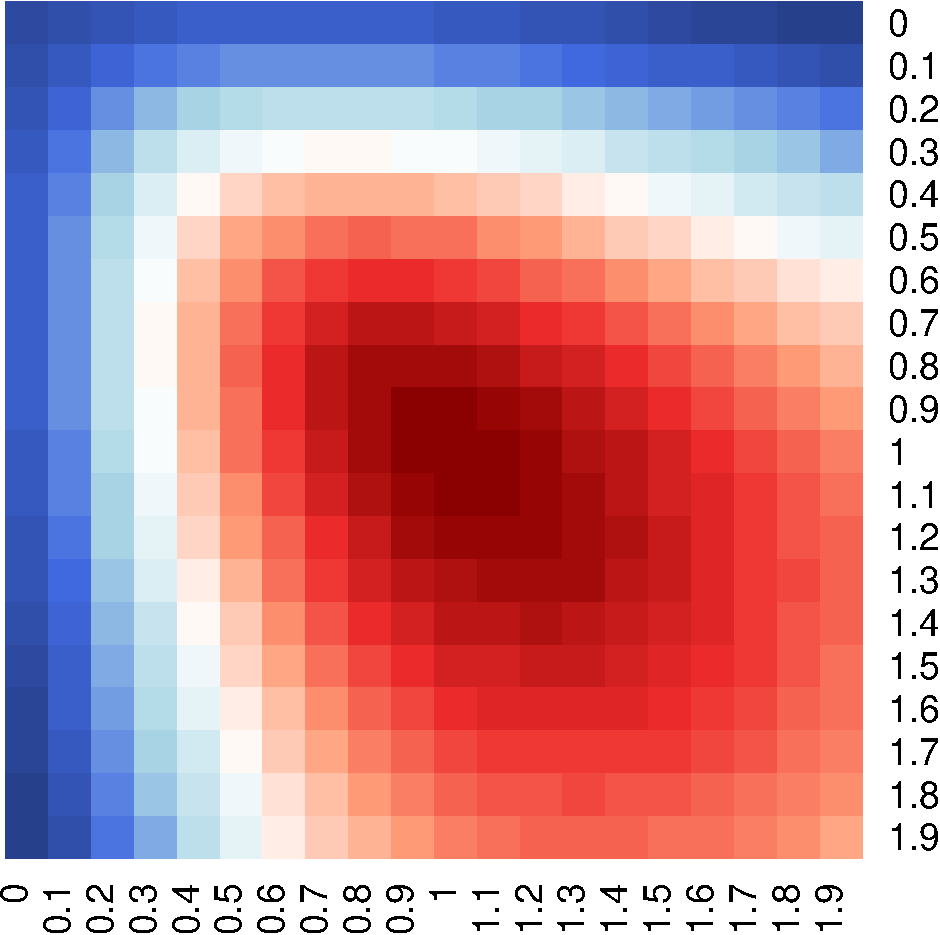
\includegraphics[width=0.33\textwidth]{sigma_marg_alpha=50.pdf}
 	}
 \caption{Interaction effect of agent parameters $\alpha$ and $\sigma$.}
 \label{figure:sigma-marg-alpha}
\end{figure}

\section{ESS analysis}

In chapter \ref{chapter:vagueness-pragmatics}, a definition of an evolutionary stable strategy (ESS) was given, which I will call "strong ESS" from now on. For short recap,  strategy $s_i$ is a "strong ESS", if for all $s_j \neq s_i \in  S$:
\begin{align}
\label{eq:strongESS}
EU(s_i, s_j) &> EU(s_j, s_j)
\end{align}
Each of the 2000 types of agents is checked to be a strong ESS, with the following result: After the latter definition, only $type_{opt} = \big[ \mu=0.8, \sigma=0.5, \alpha=100 \big] $ is an ESS. This allows to omit examination of evolutionary dynamics at this point, because at the end the best strategy will still be of $type_{opt}$.\\

The choice of the set of possible alphas $A$ does have an effect on the ESS analysis. For $A = \{1, 5, 10, 50\}$ the result looks similar, the only strong ESS is $type = \big[ \mu=0.8, \sigma=0.5, \alpha=50 \big]$.
Apparently, if e.g. $A = \{1, 5, 10\}$, no "strong ESS" after Eq.\ref{eq:strongESS} can be found. 
Instead, a list of "weak ESS" can be received. For strategy $s_i$ to be a "weak ESS", the following conditions have to be met, specified by \cite{smith1973logic}:\\

For all $s_j \neq s_i \in  S$:
\begin{align}
\label{eq:weakESS}
1. EU(s_i, s_i) &\geq EU(s_j, s_i) \quad \textbf{or} \\
2. EU(s_i, s_i) &= EU(s_j, s_i) \quad \textbf{and} \quad EU(s_i, s_j) > EU(s_j, s_j)
\end{align}
The weak ESS's are dominated by maximally rational agents and contain crisp interpretations as well as vague interpretations. A further examination could apply evolutionary dynamics to the resulting ESS after Eq.\ref{eq:weakESS}. In this work, the result of the examination of strong ESS suffices to undermine the evidence given by the main effect of $\sigma$ and the interaction effect of $\sigma$ and $\alpha$:\\

The type $type_{opt} = \big[ \mu=0.8, \sigma=0.5, \alpha=100 \big] $ is maximally rational. The optimal value for $\mu = 0.8$ seems to capture the meaning of \textit{tall} as \textit{taller than average} fairly well (with $Pr(w)$ being a standard normal distribution). The optimal degree of vagueness in the literal meaning is described by the optimal value for $\sigma = 0.5$. A rather vague interpretation leads to higher overall EU results and allows a pragmatic listener to also infer the meaning of negated vague terms. The listener strategy of the presented strong ESS type is displayed in Fig.\ref{subfig-1:L1_vague50}.\\

For future examination, one could combine the presented approach with evolutionary dynamics, such as the Replicator-Mutator dynamic, to see what strategy/type will overtake a population. Apart from that, various other extensions to the model could be made, like including joint inference over world state, type and comparison class. The RSA model provides a framework that allows to implement extensions to the model rather easily and provides interpretable results.
\chapter{Conclusion}
\label{sec:conclusion}

In this work, a computational cognitive model of language production/understanding is used to examine the effect of vague language use with the example of gradable adjectives, more specific with \textit{short}, \textit{tall} and their negations \textit{not-short} and \textit{not-tall}. A semantics for vague terms has been presented, where vagueness is defined as uncertainty about the threshold $\theta$ after which to use a word like \textit{tall}. Therefore, the vagueness considered here is actually vagueness in the literal meaning, that gets resolved by each agent individually, depending on their \textit{type}. Each type consists of the parameters $\mu$, $\sigma$ and $\alpha$. $\mu$ is the belief about the mean value of $\theta$, while $\sigma$ indicates the uncertainty about the exact value of $\theta$. $\alpha$ works as a "rationality" parameter, determining how close the message choice of the speaker approximates the optimal utility for the listener.\\

Speaker and listener strategies in a sender-receiver game are quantified by a pragmatic model of bounded rationality, the RSA model. Rational in this sense means that the choices of messages on the speaker side and the inference of world states on the receiver side is done with respect to alternative utterances that could have been used.
Also, the prior expectation about the "norm" of a world state like e.g. the height of people is taken into account for interpretation. The space of world states is not restricted but inflected with a probability distribution over possible world states.
The scale in the present simulation can be interpreted as "deviation from the norm". Therefore it also allows to explain the different meaning of \textit{tall} for different comparison classes (tall girl, tall mountain, ...).\\

The RSA model has been used in many applications for successfully predicting linguistic phenomena like e.g. scale implicatures, although it has been criticized to be unrealistic because it is assuming that people are more rational than they actually are. While it is true to say it is unrealistic that people perform complex mathematical probabilistic computations in their mind before choosing or interpreting a message, it still seems to be the case that human cognition is making use of probabilistic heuristics, e.g. in recursive reasoning. Another disadvantage of the RSA model is that it requires a hand-built lexicon with implemented semantic meaning. \cite{monroe2015learning} suggested an extension to the model by combining it with a machine learning approach, that "removes the need to specify a complex semantic lexicon by hand". In this work the semantics of the messages are highly important, as the key feature of "vagueness" is embedded in the literal semantic meaning. Therefore it is necessary in this case to specify the lexicon by hand, to examine the effect of language features in the literal meaning.\\

The measures of communicative success of a pair of agents with different strategies/types are the expected utility score as well as the examination of evolutionary stable strategies.
The EU results show interesting main effects of the parameters $\sigma$ and $\alpha$, as well as an interaction effect. More rational agents (with a high value for $\alpha$ in their type) perform better than irrational agents (with a low $\alpha$ value).\\

One of the most interesting findings is that the $\sigma$ value that leads to the best EU results holds a significant amount of vagueness in the literal meaning. The interaction effect between $\alpha$ and $\sigma$ shows that a rational agent prefers vague interpretation of messages over crisp ones, while it is the other way round for irrational agents.
This underlines Wright's (1976, page 154) observation that "the utility and point of the classifications expressed by many vague predicates would be frustrated if they were supplied with sharp boundaries". The best strategy (the ESS) shows specific posterior distribution patterns, i.e. a partitioning of the state space over the messages. Furthermore, the ordering of the interpretation of the categories that are inferred for the negations of gradable adjectives is the same as predicted from \cite{tesslernot}.\\

Finally, it seems that the cognitive ability of pragmatic recursive reasoning enables us to infer useful interpretations of vague adjectives even beyond their literal meaning. Therefore, the results of the RSA model give a suggestion for explaining the prevalence of vague terms in natural language use for rational individuals. Vagueness indeed seems to be rational.







%\appendix
%\chapter{Code of RSA-Model and Simulation}

\bibliography{bibliography}

\end{document}

